\documentclass[conference]{IEEEtran}
\IEEEoverridecommandlockouts
\usepackage{cite}
\usepackage{amsmath,amssymb,amsfonts}
\usepackage{graphicx}
\usepackage{textcomp}
\usepackage{xcolor}
\usepackage{booktabs}
\usepackage[hyphens]{url}
\usepackage[hidelinks,breaklinks=true]{hyperref}

% Every number in the prose is \R{key}, generated from the analysis outputs by
% 16_RESULTS/analysis/make_numbers.py; tables are generated by make_latex_tables.py.
% No number in this manuscript is typed by hand.
% Generated by 16_RESULTS/analysis/make_numbers.py. Do not edit by hand.
\makeatletter
\newcommand{\R}[1]{\ifcsname res@#1\endcsname\csname res@#1\endcsname\else\textbf{??#1}\PackageWarning{numbers}{Unknown result key #1}\fi}
\expandafter\def\csname res@agree.judge\endcsname{70.6}
\expandafter\def\csname res@agree.rules\endcsname{89.5}
\expandafter\def\csname res@agree.self\endcsname{93.8}
\expandafter\def\csname res@ai.llm.nonp5\endcsname{61}
\expandafter\def\csname res@ai.llm.p5\endcsname{20}
\expandafter\def\csname res@ai.llm.svsi\endcsname{81}
\expandafter\def\csname res@ai.nonp5\endcsname{114}
\expandafter\def\csname res@ai.p5\endcsname{20}
\expandafter\def\csname res@ai.svsi\endcsname{134}
\expandafter\def\csname res@ann.items\endcsname{200}
\expandafter\def\csname res@ann.median_s\endcsname{3}
\expandafter\def\csname res@ann.minutes\endcsname{33}
\expandafter\def\csname res@ann.repeats\endcsname{20}
\expandafter\def\csname res@c.A.ci\endcsname{1.7--8.7}
\expandafter\def\csname res@c.A.rate\endcsname{3.8}
\expandafter\def\csname res@c.A.struct\endcsname{97.8}
\expandafter\def\csname res@c.B.ci\endcsname{48.2--58.4}
\expandafter\def\csname res@c.B.rate\endcsname{53.3}
\expandafter\def\csname res@c.B.struct\endcsname{93.6}
\expandafter\def\csname res@c.C.ci\endcsname{58.4--78.1}
\expandafter\def\csname res@c.C.rate\endcsname{69.1}
\expandafter\def\csname res@c.C.struct\endcsname{96.5}
\expandafter\def\csname res@c.D.ci\endcsname{33.7--41.9}
\expandafter\def\csname res@c.D.rate\endcsname{37.7}
\expandafter\def\csname res@c.D.struct\endcsname{84.0}
\expandafter\def\csname res@c.E.ci\endcsname{21.1--28.2}
\expandafter\def\csname res@c.E.rate\endcsname{24.5}
\expandafter\def\csname res@c.E.struct\endcsname{92.8}
\expandafter\def\csname res@c.F.ci\endcsname{22.9--42.9}
\expandafter\def\csname res@c.F.rate\endcsname{32.1}
\expandafter\def\csname res@c.F.struct\endcsname{96.5}
\expandafter\def\csname res@c.G.ci\endcsname{11.6--24.7}
\expandafter\def\csname res@c.G.rate\endcsname{17.2}
\expandafter\def\csname res@c.G.struct\endcsname{100.0}
\expandafter\def\csname res@cat.aifacing\endcsname{44}
\expandafter\def\csname res@cat.crossfield\endcsname{45}
\expandafter\def\csname res@cat.financial\endcsname{12}
\expandafter\def\csname res@cat.freetext\endcsname{51}
\expandafter\def\csname res@cat.search\endcsname{32}
\expandafter\def\csname res@cat.simple\endcsname{27}
\expandafter\def\csname res@cat.structured\endcsname{57}
\expandafter\def\csname res@cmh.CvB.ci\endcsname{1.20--3.95}
\expandafter\def\csname res@cmh.CvB.or\endcsname{2.18}
\expandafter\def\csname res@cmh.CvB.p\endcsname{$p=0.004$}
\expandafter\def\csname res@cmh.DvB.ci\endcsname{0.34--0.66}
\expandafter\def\csname res@cmh.DvB.or\endcsname{0.47}
\expandafter\def\csname res@cmh.DvB.p\endcsname{$p<0.001$}
\expandafter\def\csname res@cmh.EvB.ci\endcsname{0.11--0.23}
\expandafter\def\csname res@cmh.EvB.or\endcsname{0.16}
\expandafter\def\csname res@cmh.EvB.p\endcsname{$p<0.001$}
\expandafter\def\csname res@cmh.EvD.ci\endcsname{0.15--0.35}
\expandafter\def\csname res@cmh.EvD.or\endcsname{0.23}
\expandafter\def\csname res@cmh.EvD.p\endcsname{$p<0.001$}
\expandafter\def\csname res@cmh.EvD.reduction\endcsname{77}
\expandafter\def\csname res@cmh.EvG.ci\endcsname{0.77--2.27}
\expandafter\def\csname res@cmh.EvG.or\endcsname{1.32}
\expandafter\def\csname res@cmh.EvG.p\endcsname{$p=0.29$}
\expandafter\def\csname res@e1.decided\endcsname{1876}
\expandafter\def\csname res@e1.failcallerror\endcsname{75}
\expandafter\def\csname res@e1.failcells\endcsname{52}
\expandafter\def\csname res@e1.failrecords\endcsname{88}
\expandafter\def\csname res@e1.failunparse\endcsname{13}
\expandafter\def\csname res@e1.inputs\endcsname{3881}
\expandafter\def\csname res@e1.keymismatch\endcsname{430}
\expandafter\def\csname res@e1.p5\endcsname{74}
\expandafter\def\csname res@e1.passes\endcsname{2917}
\expandafter\def\csname res@e1.primary\endcsname{3236}
\expandafter\def\csname res@e1.refdrafted\endcsname{272}
\expandafter\def\csname res@e1.refvalues\endcsname{275}
\expandafter\def\csname res@e1.retried\endcsname{131}
\expandafter\def\csname res@e1.reviewexcluded\endcsname{10}
\expandafter\def\csname res@e1.undecided\endcsname{1041}
\expandafter\def\csname res@e1.undecided.unjudged\endcsname{1001}
\expandafter\def\csname res@e1.undecided.unsure\endcsname{40}
\expandafter\def\csname res@e2b.large.all\endcsname{23.1}
\expandafter\def\csname res@e2b.large.all.or\endcsname{1.0}
\expandafter\def\csname res@e2b.large.all.p\endcsname{$p_{\mathrm{Holm}}=0.90$}
\expandafter\def\csname res@e2b.large.obj\endcsname{1.4}
\expandafter\def\csname res@e2b.large.obj.or\endcsname{1.3}
\expandafter\def\csname res@e2b.large.obj.p\endcsname{$p_{\mathrm{Holm}}=0.77$}
\expandafter\def\csname res@e2b.ref.all\endcsname{22.3}
\expandafter\def\csname res@e2b.ref.obj\endcsname{1.1}
\expandafter\def\csname res@e2b.small.all\endcsname{35.0}
\expandafter\def\csname res@e2b.small.all.or\endcsname{1.9}
\expandafter\def\csname res@e2b.small.all.p\endcsname{$p_{\mathrm{Holm}}=0.02$}
\expandafter\def\csname res@e2b.small.obj\endcsname{4.8}
\expandafter\def\csname res@e2b.small.obj.or\endcsname{4.4}
\expandafter\def\csname res@e2b.small.obj.p\endcsname{$p_{\mathrm{Holm}}=0.001$}
\expandafter\def\csname res@e2b.tzero.all\endcsname{26.3}
\expandafter\def\csname res@e2b.tzero.all.or\endcsname{1.2}
\expandafter\def\csname res@e2b.tzero.all.p\endcsname{$p_{\mathrm{Holm}}=0.84$}
\expandafter\def\csname res@e2b.tzero.obj\endcsname{2.8}
\expandafter\def\csname res@e2b.tzero.obj.or\endcsname{2.5}
\expandafter\def\csname res@e2b.tzero.obj.p\endcsname{$p_{\mathrm{Holm}}=0.15$}
\expandafter\def\csname res@e3.EMB.auroc\endcsname{0.45}
\expandafter\def\csname res@e3.EMB.ci\endcsname{2.2--7.3}
\expandafter\def\csname res@e3.EMB.fpr\endcsname{5.6}
\expandafter\def\csname res@e3.EMB.fprG\endcsname{4.8}
\expandafter\def\csname res@e3.EMB.fullrecall\endcsname{3.2}
\expandafter\def\csname res@e3.EMB.nfpr\endcsname{2.1}
\expandafter\def\csname res@e3.EMB.noverdict\endcsname{0}
\expandafter\def\csname res@e3.EMB.nrecall\endcsname{1.7}
\expandafter\def\csname res@e3.EMB.recall\endcsname{4.7}
\expandafter\def\csname res@e3.EMB.rjud\endcsname{6.5}
\expandafter\def\csname res@e3.EMB.robj\endcsname{0.0}
\expandafter\def\csname res@e3.HYB.auroc\endcsname{0.60}
\expandafter\def\csname res@e3.HYB.ci\endcsname{21.3--32.5}
\expandafter\def\csname res@e3.HYB.fpr\endcsname{5.6}
\expandafter\def\csname res@e3.HYB.fprG\endcsname{4.8}
\expandafter\def\csname res@e3.HYB.fullrecall\endcsname{36.6}
\expandafter\def\csname res@e3.HYB.nfpr\endcsname{2.1}
\expandafter\def\csname res@e3.HYB.noverdict\endcsname{0}
\expandafter\def\csname res@e3.HYB.nrecall\endcsname{24.2}
\expandafter\def\csname res@e3.HYB.recall\endcsname{27.1}
\expandafter\def\csname res@e3.HYB.rjud\endcsname{6.5}
\expandafter\def\csname res@e3.HYB.robj\endcsname{100.0}
\expandafter\def\csname res@e3.JUDGE.auroc\endcsname{0.76}
\expandafter\def\csname res@e3.JUDGE.ci\endcsname{18.5--29.4}
\expandafter\def\csname res@e3.JUDGE.fpr\endcsname{3.5}
\expandafter\def\csname res@e3.JUDGE.fprG\endcsname{1.6}
\expandafter\def\csname res@e3.JUDGE.nfpr\endcsname{6.8}
\expandafter\def\csname res@e3.JUDGE.noverdict\endcsname{26}
\expandafter\def\csname res@e3.JUDGE.nrecall\endcsname{51.7}
\expandafter\def\csname res@e3.JUDGE.recall\endcsname{23.7}
\expandafter\def\csname res@e3.JUDGE.rjud\endcsname{22.4}
\expandafter\def\csname res@e3.JUDGE.robj\endcsname{24.5}
\expandafter\def\csname res@e3.R.auroc\endcsname{0.61}
\expandafter\def\csname res@e3.R.ci\endcsname{17.0--27.8}
\expandafter\def\csname res@e3.R.fpr\endcsname{0.0}
\expandafter\def\csname res@e3.R.fprG\endcsname{0.0}
\expandafter\def\csname res@e3.R.fullrecall\endcsname{33.3}
\expandafter\def\csname res@e3.R.nfpr\endcsname{0.0}
\expandafter\def\csname res@e3.R.noverdict\endcsname{0}
\expandafter\def\csname res@e3.R.nrecall\endcsname{22.5}
\expandafter\def\csname res@e3.R.recall\endcsname{22.5}
\expandafter\def\csname res@e3.R.rjud\endcsname{0.0}
\expandafter\def\csname res@e3.R.robj\endcsname{100.0}
\expandafter\def\csname res@e3.SLM.auroc\endcsname{0.75}
\expandafter\def\csname res@e3.SLM.ci\endcsname{0.0--2.9}
\expandafter\def\csname res@e3.SLM.fpr\endcsname{1.2}
\expandafter\def\csname res@e3.SLM.fprG\endcsname{1.6}
\expandafter\def\csname res@e3.SLM.nfpr\endcsname{20.1}
\expandafter\def\csname res@e3.SLM.noverdict\endcsname{0}
\expandafter\def\csname res@e3.SLM.nrecall\endcsname{69.1}
\expandafter\def\csname res@e3.SLM.recall\endcsname{1.3}
\expandafter\def\csname res@e3.SLM.rjud\endcsname{0.6}
\expandafter\def\csname res@e3.SLM.robj\endcsname{3.8}
\expandafter\def\csname res@e3.emb.foldfprmax\endcsname{30}
\expandafter\def\csname res@e3.fulln\endcsname{1937}
\expandafter\def\csname res@e3.n\endcsname{575}
\expandafter\def\csname res@e3.neg\endcsname{339}
\expandafter\def\csname res@e3.pos\endcsname{236}
\expandafter\def\csname res@e4.EMB.c1.courses.addedp50\endcsname{27}
\expandafter\def\csname res@e4.EMB.c1.courses.addedp975\endcsname{65}
\expandafter\def\csname res@e4.EMB.c1.courses.p50\endcsname{47}
\expandafter\def\csname res@e4.EMB.c1.courses.p975\endcsname{93}
\expandafter\def\csname res@e4.EMB.c1.courses.rps\endcsname{19.2}
\expandafter\def\csname res@e4.EMB.c1.maxadd\endcsname{96}
\expandafter\def\csname res@e4.EMB.c1.maxp50add\endcsname{48}
\expandafter\def\csname res@e4.EMB.c1.maxp50add.s\endcsname{0.0}
\expandafter\def\csname res@e4.EMB.c1.minadd\endcsname{65}
\expandafter\def\csname res@e4.EMB.c1.minp50add\endcsname{27}
\expandafter\def\csname res@e4.EMB.c1.minp50add.s\endcsname{0.0}
\expandafter\def\csname res@e4.EMB.c1.profile.addedp50\endcsname{36}
\expandafter\def\csname res@e4.EMB.c1.profile.addedp975\endcsname{70}
\expandafter\def\csname res@e4.EMB.c1.profile.p50\endcsname{57}
\expandafter\def\csname res@e4.EMB.c1.profile.p975\endcsname{102}
\expandafter\def\csname res@e4.EMB.c1.profile.rps\endcsname{15.9}
\expandafter\def\csname res@e4.EMB.c1.reviews.addedp50\endcsname{48}
\expandafter\def\csname res@e4.EMB.c1.reviews.addedp975\endcsname{96}
\expandafter\def\csname res@e4.EMB.c1.reviews.p50\endcsname{68}
\expandafter\def\csname res@e4.EMB.c1.reviews.p975\endcsname{127}
\expandafter\def\csname res@e4.EMB.c1.reviews.rps\endcsname{13.2}
\expandafter\def\csname res@e4.EMB.c8.courses.addedp50\endcsname{126}
\expandafter\def\csname res@e4.EMB.c8.courses.addedp975\endcsname{122}
\expandafter\def\csname res@e4.EMB.c8.courses.p50\endcsname{272}
\expandafter\def\csname res@e4.EMB.c8.courses.p975\endcsname{444}
\expandafter\def\csname res@e4.EMB.c8.courses.rps\endcsname{27.9}
\expandafter\def\csname res@e4.EMB.c8.maxadd\endcsname{751}
\expandafter\def\csname res@e4.EMB.c8.maxp50add\endcsname{288}
\expandafter\def\csname res@e4.EMB.c8.maxp50add.s\endcsname{0.3}
\expandafter\def\csname res@e4.EMB.c8.minadd\endcsname{122}
\expandafter\def\csname res@e4.EMB.c8.minp50add\endcsname{126}
\expandafter\def\csname res@e4.EMB.c8.minp50add.s\endcsname{0.1}
\expandafter\def\csname res@e4.EMB.c8.profile.addedp50\endcsname{199}
\expandafter\def\csname res@e4.EMB.c8.profile.addedp975\endcsname{310}
\expandafter\def\csname res@e4.EMB.c8.profile.p50\endcsname{355}
\expandafter\def\csname res@e4.EMB.c8.profile.p975\endcsname{787}
\expandafter\def\csname res@e4.EMB.c8.profile.rps\endcsname{20.6}
\expandafter\def\csname res@e4.EMB.c8.reviews.addedp50\endcsname{288}
\expandafter\def\csname res@e4.EMB.c8.reviews.addedp975\endcsname{751}
\expandafter\def\csname res@e4.EMB.c8.reviews.p50\endcsname{443}
\expandafter\def\csname res@e4.EMB.c8.reviews.p975\endcsname{1084}
\expandafter\def\csname res@e4.EMB.c8.reviews.rps\endcsname{16.0}
\expandafter\def\csname res@e4.HYB.c1.courses.addedp50\endcsname{26}
\expandafter\def\csname res@e4.HYB.c1.courses.addedp975\endcsname{65}
\expandafter\def\csname res@e4.HYB.c1.courses.p50\endcsname{46}
\expandafter\def\csname res@e4.HYB.c1.courses.p975\endcsname{93}
\expandafter\def\csname res@e4.HYB.c1.courses.rps\endcsname{19.2}
\expandafter\def\csname res@e4.HYB.c1.maxadd\endcsname{82}
\expandafter\def\csname res@e4.HYB.c1.maxp50add\endcsname{45}
\expandafter\def\csname res@e4.HYB.c1.maxp50add.s\endcsname{0.0}
\expandafter\def\csname res@e4.HYB.c1.minadd\endcsname{65}
\expandafter\def\csname res@e4.HYB.c1.minp50add\endcsname{26}
\expandafter\def\csname res@e4.HYB.c1.minp50add.s\endcsname{0.0}
\expandafter\def\csname res@e4.HYB.c1.profile.addedp50\endcsname{37}
\expandafter\def\csname res@e4.HYB.c1.profile.addedp975\endcsname{68}
\expandafter\def\csname res@e4.HYB.c1.profile.p50\endcsname{58}
\expandafter\def\csname res@e4.HYB.c1.profile.p975\endcsname{100}
\expandafter\def\csname res@e4.HYB.c1.profile.rps\endcsname{15.6}
\expandafter\def\csname res@e4.HYB.c1.reviews.addedp50\endcsname{45}
\expandafter\def\csname res@e4.HYB.c1.reviews.addedp975\endcsname{82}
\expandafter\def\csname res@e4.HYB.c1.reviews.p50\endcsname{65}
\expandafter\def\csname res@e4.HYB.c1.reviews.p975\endcsname{113}
\expandafter\def\csname res@e4.HYB.c1.reviews.rps\endcsname{13.6}
\expandafter\def\csname res@e4.HYB.c8.courses.addedp50\endcsname{103}
\expandafter\def\csname res@e4.HYB.c8.courses.addedp975\endcsname{131}
\expandafter\def\csname res@e4.HYB.c8.courses.p50\endcsname{249}
\expandafter\def\csname res@e4.HYB.c8.courses.p975\endcsname{453}
\expandafter\def\csname res@e4.HYB.c8.courses.rps\endcsname{29.0}
\expandafter\def\csname res@e4.HYB.c8.maxadd\endcsname{396}
\expandafter\def\csname res@e4.HYB.c8.maxp50add\endcsname{270}
\expandafter\def\csname res@e4.HYB.c8.maxp50add.s\endcsname{0.3}
\expandafter\def\csname res@e4.HYB.c8.minadd\endcsname{131}
\expandafter\def\csname res@e4.HYB.c8.minp50add\endcsname{103}
\expandafter\def\csname res@e4.HYB.c8.minp50add.s\endcsname{0.1}
\expandafter\def\csname res@e4.HYB.c8.profile.addedp50\endcsname{169}
\expandafter\def\csname res@e4.HYB.c8.profile.addedp975\endcsname{275}
\expandafter\def\csname res@e4.HYB.c8.profile.p50\endcsname{325}
\expandafter\def\csname res@e4.HYB.c8.profile.p975\endcsname{752}
\expandafter\def\csname res@e4.HYB.c8.profile.rps\endcsname{22.9}
\expandafter\def\csname res@e4.HYB.c8.reviews.addedp50\endcsname{270}
\expandafter\def\csname res@e4.HYB.c8.reviews.addedp975\endcsname{396}
\expandafter\def\csname res@e4.HYB.c8.reviews.p50\endcsname{425}
\expandafter\def\csname res@e4.HYB.c8.reviews.p975\endcsname{729}
\expandafter\def\csname res@e4.HYB.c8.reviews.rps\endcsname{17.7}
\expandafter\def\csname res@e4.JUDGE.c1.courses.addedp50\endcsname{7165}
\expandafter\def\csname res@e4.JUDGE.c1.courses.addedp975\endcsname{10186}
\expandafter\def\csname res@e4.JUDGE.c1.courses.p50\endcsname{7185}
\expandafter\def\csname res@e4.JUDGE.c1.courses.p975\endcsname{10214}
\expandafter\def\csname res@e4.JUDGE.c1.courses.rps\endcsname{0.1}
\expandafter\def\csname res@e4.JUDGE.c1.maxadd\endcsname{10824}
\expandafter\def\csname res@e4.JUDGE.c1.maxp50add\endcsname{7704}
\expandafter\def\csname res@e4.JUDGE.c1.maxp50add.s\endcsname{7.7}
\expandafter\def\csname res@e4.JUDGE.c1.minadd\endcsname{7683}
\expandafter\def\csname res@e4.JUDGE.c1.minp50add\endcsname{1611}
\expandafter\def\csname res@e4.JUDGE.c1.minp50add.s\endcsname{1.6}
\expandafter\def\csname res@e4.JUDGE.c1.profile.addedp50\endcsname{1611}
\expandafter\def\csname res@e4.JUDGE.c1.profile.addedp975\endcsname{7683}
\expandafter\def\csname res@e4.JUDGE.c1.profile.p50\endcsname{1632}
\expandafter\def\csname res@e4.JUDGE.c1.profile.p975\endcsname{7715}
\expandafter\def\csname res@e4.JUDGE.c1.profile.rps\endcsname{0.5}
\expandafter\def\csname res@e4.JUDGE.c1.reviews.addedp50\endcsname{7704}
\expandafter\def\csname res@e4.JUDGE.c1.reviews.addedp975\endcsname{10824}
\expandafter\def\csname res@e4.JUDGE.c1.reviews.p50\endcsname{7724}
\expandafter\def\csname res@e4.JUDGE.c1.reviews.p975\endcsname{10855}
\expandafter\def\csname res@e4.JUDGE.c1.reviews.rps\endcsname{0.1}
\expandafter\def\csname res@e4.JUDGE.c8.courses.addedp50\endcsname{$>$60\,000}
\expandafter\def\csname res@e4.JUDGE.c8.courses.addedp975\endcsname{$>$60\,000}
\expandafter\def\csname res@e4.JUDGE.c8.courses.p50\endcsname{$>$60\,000}
\expandafter\def\csname res@e4.JUDGE.c8.courses.p975\endcsname{$>$60\,000}
\expandafter\def\csname res@e4.JUDGE.c8.courses.rps\endcsname{0.0}
\expandafter\def\csname res@e4.JUDGE.c8.maxadd\endcsname{$>$60\,000}
\expandafter\def\csname res@e4.JUDGE.c8.maxp50add\endcsname{$>$60\,000}
\expandafter\def\csname res@e4.JUDGE.c8.maxp50add.s\endcsname{$>$60}
\expandafter\def\csname res@e4.JUDGE.c8.minadd\endcsname{23474}
\expandafter\def\csname res@e4.JUDGE.c8.minp50add\endcsname{14282}
\expandafter\def\csname res@e4.JUDGE.c8.minp50add.s\endcsname{14.3}
\expandafter\def\csname res@e4.JUDGE.c8.profile.addedp50\endcsname{14282}
\expandafter\def\csname res@e4.JUDGE.c8.profile.addedp975\endcsname{23474}
\expandafter\def\csname res@e4.JUDGE.c8.profile.p50\endcsname{14438}
\expandafter\def\csname res@e4.JUDGE.c8.profile.p975\endcsname{23951}
\expandafter\def\csname res@e4.JUDGE.c8.profile.rps\endcsname{0.4}
\expandafter\def\csname res@e4.JUDGE.c8.reviews.addedp50\endcsname{$>$60\,000}
\expandafter\def\csname res@e4.JUDGE.c8.reviews.addedp975\endcsname{$>$60\,000}
\expandafter\def\csname res@e4.JUDGE.c8.reviews.p50\endcsname{$>$60\,000}
\expandafter\def\csname res@e4.JUDGE.c8.reviews.p975\endcsname{$>$60\,000}
\expandafter\def\csname res@e4.JUDGE.c8.reviews.rps\endcsname{0.0}
\expandafter\def\csname res@e4.R.c1.courses.addedp50\endcsname{0}
\expandafter\def\csname res@e4.R.c1.courses.addedp975\endcsname{1}
\expandafter\def\csname res@e4.R.c1.courses.p50\endcsname{20}
\expandafter\def\csname res@e4.R.c1.courses.p975\endcsname{29}
\expandafter\def\csname res@e4.R.c1.courses.rps\endcsname{46.0}
\expandafter\def\csname res@e4.R.c1.maxadd\endcsname{1}
\expandafter\def\csname res@e4.R.c1.maxp50add\endcsname{2}
\expandafter\def\csname res@e4.R.c1.maxp50add.s\endcsname{0.0}
\expandafter\def\csname res@e4.R.c1.minadd\endcsname{0}
\expandafter\def\csname res@e4.R.c1.minp50add\endcsname{0}
\expandafter\def\csname res@e4.R.c1.minp50add.s\endcsname{0.0}
\expandafter\def\csname res@e4.R.c1.profile.addedp50\endcsname{1}
\expandafter\def\csname res@e4.R.c1.profile.addedp975\endcsname{1}
\expandafter\def\csname res@e4.R.c1.profile.p50\endcsname{22}
\expandafter\def\csname res@e4.R.c1.profile.p975\endcsname{33}
\expandafter\def\csname res@e4.R.c1.profile.rps\endcsname{41.9}
\expandafter\def\csname res@e4.R.c1.reviews.addedp50\endcsname{2}
\expandafter\def\csname res@e4.R.c1.reviews.addedp975\endcsname{0}
\expandafter\def\csname res@e4.R.c1.reviews.p50\endcsname{22}
\expandafter\def\csname res@e4.R.c1.reviews.p975\endcsname{31}
\expandafter\def\csname res@e4.R.c1.reviews.rps\endcsname{43.1}
\expandafter\def\csname res@e4.R.c8.courses.addedp50\endcsname{3}
\expandafter\def\csname res@e4.R.c8.courses.addedp975\endcsname{-5}
\expandafter\def\csname res@e4.R.c8.courses.p50\endcsname{149}
\expandafter\def\csname res@e4.R.c8.courses.p975\endcsname{317}
\expandafter\def\csname res@e4.R.c8.courses.rps\endcsname{47.6}
\expandafter\def\csname res@e4.R.c8.maxadd\endcsname{14}
\expandafter\def\csname res@e4.R.c8.maxp50add\endcsname{6}
\expandafter\def\csname res@e4.R.c8.maxp50add.s\endcsname{0.0}
\expandafter\def\csname res@e4.R.c8.minadd\endcsname{-136}
\expandafter\def\csname res@e4.R.c8.minp50add\endcsname{2}
\expandafter\def\csname res@e4.R.c8.minp50add.s\endcsname{0.0}
\expandafter\def\csname res@e4.R.c8.profile.addedp50\endcsname{2}
\expandafter\def\csname res@e4.R.c8.profile.addedp975\endcsname{-136}
\expandafter\def\csname res@e4.R.c8.profile.p50\endcsname{158}
\expandafter\def\csname res@e4.R.c8.profile.p975\endcsname{341}
\expandafter\def\csname res@e4.R.c8.profile.rps\endcsname{44.8}
\expandafter\def\csname res@e4.R.c8.reviews.addedp50\endcsname{6}
\expandafter\def\csname res@e4.R.c8.reviews.addedp975\endcsname{14}
\expandafter\def\csname res@e4.R.c8.reviews.p50\endcsname{161}
\expandafter\def\csname res@e4.R.c8.reviews.p975\endcsname{347}
\expandafter\def\csname res@e4.R.c8.reviews.rps\endcsname{43.9}
\expandafter\def\csname res@e4.SLM.c1.courses.addedp50\endcsname{527}
\expandafter\def\csname res@e4.SLM.c1.courses.addedp975\endcsname{761}
\expandafter\def\csname res@e4.SLM.c1.courses.p50\endcsname{547}
\expandafter\def\csname res@e4.SLM.c1.courses.p975\endcsname{789}
\expandafter\def\csname res@e4.SLM.c1.courses.rps\endcsname{1.8}
\expandafter\def\csname res@e4.SLM.c1.maxadd\endcsname{761}
\expandafter\def\csname res@e4.SLM.c1.maxp50add\endcsname{534}
\expandafter\def\csname res@e4.SLM.c1.maxp50add.s\endcsname{0.5}
\expandafter\def\csname res@e4.SLM.c1.minadd\endcsname{655}
\expandafter\def\csname res@e4.SLM.c1.minp50add\endcsname{527}
\expandafter\def\csname res@e4.SLM.c1.minp50add.s\endcsname{0.5}
\expandafter\def\csname res@e4.SLM.c1.profile.addedp50\endcsname{531}
\expandafter\def\csname res@e4.SLM.c1.profile.addedp975\endcsname{655}
\expandafter\def\csname res@e4.SLM.c1.profile.p50\endcsname{552}
\expandafter\def\csname res@e4.SLM.c1.profile.p975\endcsname{687}
\expandafter\def\csname res@e4.SLM.c1.profile.rps\endcsname{1.8}
\expandafter\def\csname res@e4.SLM.c1.reviews.addedp50\endcsname{534}
\expandafter\def\csname res@e4.SLM.c1.reviews.addedp975\endcsname{698}
\expandafter\def\csname res@e4.SLM.c1.reviews.p50\endcsname{554}
\expandafter\def\csname res@e4.SLM.c1.reviews.p975\endcsname{729}
\expandafter\def\csname res@e4.SLM.c1.reviews.rps\endcsname{1.7}
\expandafter\def\csname res@e4.SLM.c8.courses.addedp50\endcsname{4149}
\expandafter\def\csname res@e4.SLM.c8.courses.addedp975\endcsname{6856}
\expandafter\def\csname res@e4.SLM.c8.courses.p50\endcsname{4295}
\expandafter\def\csname res@e4.SLM.c8.courses.p975\endcsname{7178}
\expandafter\def\csname res@e4.SLM.c8.courses.rps\endcsname{1.7}
\expandafter\def\csname res@e4.SLM.c8.maxadd\endcsname{7180}
\expandafter\def\csname res@e4.SLM.c8.maxp50add\endcsname{4210}
\expandafter\def\csname res@e4.SLM.c8.maxp50add.s\endcsname{4.2}
\expandafter\def\csname res@e4.SLM.c8.minadd\endcsname{6780}
\expandafter\def\csname res@e4.SLM.c8.minp50add\endcsname{4149}
\expandafter\def\csname res@e4.SLM.c8.minp50add.s\endcsname{4.1}
\expandafter\def\csname res@e4.SLM.c8.profile.addedp50\endcsname{4198}
\expandafter\def\csname res@e4.SLM.c8.profile.addedp975\endcsname{6780}
\expandafter\def\csname res@e4.SLM.c8.profile.p50\endcsname{4354}
\expandafter\def\csname res@e4.SLM.c8.profile.p975\endcsname{7257}
\expandafter\def\csname res@e4.SLM.c8.profile.rps\endcsname{1.7}
\expandafter\def\csname res@e4.SLM.c8.reviews.addedp50\endcsname{4210}
\expandafter\def\csname res@e4.SLM.c8.reviews.addedp975\endcsname{7180}
\expandafter\def\csname res@e4.SLM.c8.reviews.p50\endcsname{4365}
\expandafter\def\csname res@e4.SLM.c8.reviews.p975\endcsname{7513}
\expandafter\def\csname res@e4.SLM.c8.reviews.rps\endcsname{1.7}
\expandafter\def\csname res@e4.structural.c1.courses.addedp50\endcsname{0}
\expandafter\def\csname res@e4.structural.c1.courses.addedp975\endcsname{0}
\expandafter\def\csname res@e4.structural.c1.courses.p50\endcsname{20}
\expandafter\def\csname res@e4.structural.c1.courses.p975\endcsname{28}
\expandafter\def\csname res@e4.structural.c1.courses.rps\endcsname{47.4}
\expandafter\def\csname res@e4.structural.c1.maxadd\endcsname{0}
\expandafter\def\csname res@e4.structural.c1.maxp50add\endcsname{0}
\expandafter\def\csname res@e4.structural.c1.maxp50add.s\endcsname{0.0}
\expandafter\def\csname res@e4.structural.c1.minadd\endcsname{0}
\expandafter\def\csname res@e4.structural.c1.minp50add\endcsname{0}
\expandafter\def\csname res@e4.structural.c1.minp50add.s\endcsname{0.0}
\expandafter\def\csname res@e4.structural.c1.profile.addedp50\endcsname{0}
\expandafter\def\csname res@e4.structural.c1.profile.addedp975\endcsname{0}
\expandafter\def\csname res@e4.structural.c1.profile.p50\endcsname{21}
\expandafter\def\csname res@e4.structural.c1.profile.p975\endcsname{32}
\expandafter\def\csname res@e4.structural.c1.profile.rps\endcsname{42.9}
\expandafter\def\csname res@e4.structural.c1.reviews.addedp50\endcsname{0}
\expandafter\def\csname res@e4.structural.c1.reviews.addedp975\endcsname{0}
\expandafter\def\csname res@e4.structural.c1.reviews.p50\endcsname{20}
\expandafter\def\csname res@e4.structural.c1.reviews.p975\endcsname{31}
\expandafter\def\csname res@e4.structural.c1.reviews.rps\endcsname{45.6}
\expandafter\def\csname res@e4.structural.c8.courses.addedp50\endcsname{0}
\expandafter\def\csname res@e4.structural.c8.courses.addedp975\endcsname{0}
\expandafter\def\csname res@e4.structural.c8.courses.p50\endcsname{146}
\expandafter\def\csname res@e4.structural.c8.courses.p975\endcsname{322}
\expandafter\def\csname res@e4.structural.c8.courses.rps\endcsname{48.3}
\expandafter\def\csname res@e4.structural.c8.maxadd\endcsname{0}
\expandafter\def\csname res@e4.structural.c8.maxp50add\endcsname{0}
\expandafter\def\csname res@e4.structural.c8.maxp50add.s\endcsname{0.0}
\expandafter\def\csname res@e4.structural.c8.minadd\endcsname{0}
\expandafter\def\csname res@e4.structural.c8.minp50add\endcsname{0}
\expandafter\def\csname res@e4.structural.c8.minp50add.s\endcsname{0.0}
\expandafter\def\csname res@e4.structural.c8.profile.addedp50\endcsname{0}
\expandafter\def\csname res@e4.structural.c8.profile.addedp975\endcsname{0}
\expandafter\def\csname res@e4.structural.c8.profile.p50\endcsname{156}
\expandafter\def\csname res@e4.structural.c8.profile.p975\endcsname{477}
\expandafter\def\csname res@e4.structural.c8.profile.rps\endcsname{41.7}
\expandafter\def\csname res@e4.structural.c8.reviews.addedp50\endcsname{0}
\expandafter\def\csname res@e4.structural.c8.reviews.addedp975\endcsname{0}
\expandafter\def\csname res@e4.structural.c8.reviews.p50\endcsname{155}
\expandafter\def\csname res@e4.structural.c8.reviews.p975\endcsname{333}
\expandafter\def\csname res@e4.structural.c8.reviews.rps\endcsname{45.6}
\expandafter\def\csname res@fail.human.judge\endcsname{28}
\expandafter\def\csname res@fail.human.rules\endcsname{4}
\expandafter\def\csname res@fail.other.judge\endcsname{37}
\expandafter\def\csname res@fail.other.rules\endcsname{19}
\expandafter\def\csname res@fam.P1.D\endcsname{25.9}
\expandafter\def\csname res@fam.P1.DE\endcsname{20.3}
\expandafter\def\csname res@fam.P1.E\endcsname{14.4}
\expandafter\def\csname res@fam.P2.D\endcsname{36.2}
\expandafter\def\csname res@fam.P2.DE\endcsname{31.9}
\expandafter\def\csname res@fam.P2.E\endcsname{26.1}
\expandafter\def\csname res@fam.P3.D\endcsname{48.1}
\expandafter\def\csname res@fam.P3.DE\endcsname{43.3}
\expandafter\def\csname res@fam.P3.E\endcsname{39.1}
\expandafter\def\csname res@fam.P4.D\endcsname{29.1}
\expandafter\def\csname res@fam.P4.DE\endcsname{24.4}
\expandafter\def\csname res@fam.P4.E\endcsname{20.6}
\expandafter\def\csname res@fam.P6.D\endcsname{46.7}
\expandafter\def\csname res@fam.P6.DE\endcsname{33.1}
\expandafter\def\csname res@fam.P6.E\endcsname{22.3}
\expandafter\def\csname res@fam.P7.D\endcsname{45.6}
\expandafter\def\csname res@fam.P7.DE\endcsname{35.8}
\expandafter\def\csname res@fam.P7.E\endcsname{27.2}
\expandafter\def\csname res@h1.ci\endcsname{28.2--33.7}
\expandafter\def\csname res@h1.k\endcsname{338}
\expandafter\def\csname res@h1.n\endcsname{1094}
\expandafter\def\csname res@h1.rate\endcsname{30.9}
\expandafter\def\csname res@h1.withretried\endcsname{30.5}
\expandafter\def\csname res@h2.chi\endcsname{184.5}
\expandafter\def\csname res@h2.v\endcsname{0.31}
\expandafter\def\csname res@h3.DgtB.pholm\endcsname{1.00}
\expandafter\def\csname res@h3.EgtB.pholm\endcsname{1.00}
\expandafter\def\csname res@h3.EgtG.pholm\endcsname{0.14}
\expandafter\def\csname res@h6.part1\endcsname{fails}
\expandafter\def\csname res@h6.part2\endcsname{holds}
\expandafter\def\csname res@judge.base\endcsname{1200}
\expandafter\def\csname res@judge.supplement\endcsname{136}
\expandafter\def\csname res@kappa.judge\endcsname{0.24}
\expandafter\def\csname res@kappa.rules\endcsname{0.32}
\expandafter\def\csname res@kappa.self\endcsname{0.71}
\expandafter\def\csname res@n.judge\endcsname{126}
\expandafter\def\csname res@n.rules\endcsname{143}
\expandafter\def\csname res@n.self\endcsname{32}
\expandafter\def\csname res@newref.passes\endcsname{0}
\expandafter\def\csname res@noverdict.judge\endcsname{36}
\expandafter\def\csname res@noverdict.rules\endcsname{12}
\expandafter\def\csname res@review.change\endcsname{3}
\expandafter\def\csname res@review.delete\endcsname{7}
\expandafter\def\csname res@review.keep\endcsname{262}
\expandafter\def\csname res@review.median_s\endcsname{1}
\expandafter\def\csname res@review.minutes\endcsname{19}
\expandafter\def\csname res@rule.B-CO-2\endcsname{146}
\expandafter\def\csname res@rule.B-CO-3\endcsname{57}
\expandafter\def\csname res@rule.B-CO-7\endcsname{40}
\expandafter\def\csname res@rule.B-PR-6\endcsname{64}
\expandafter\def\csname res@rule.B-RV-3\endcsname{41}
\expandafter\def\csname res@rule.B-RV-4\endcsname{40}
\expandafter\def\csname res@rule.B-TK-4\endcsname{61}
\expandafter\def\csname res@run.D.1\endcsname{31.1}
\expandafter\def\csname res@run.D.2\endcsname{41.6}
\expandafter\def\csname res@run.D.3\endcsname{40.9}
\expandafter\def\csname res@run.E.1\endcsname{25.7}
\expandafter\def\csname res@run.E.2\endcsname{24.9}
\expandafter\def\csname res@run.E.3\endcsname{22.9}
\expandafter\def\csname res@s.B.nocontext\endcsname{36.5}
\expandafter\def\csname res@s.B.nocontext.ci\endcsname{31.7--41.7}
\expandafter\def\csname res@s.B.nodates\endcsname{50.4}
\expandafter\def\csname res@s.B.nodates.ci\endcsname{45.1--55.7}
\expandafter\def\csname res@s.B.nopthree\endcsname{53.3}
\expandafter\def\csname res@s.B.nopthree.ci\endcsname{48.2--58.4}
\expandafter\def\csname res@s.B.objective\endcsname{10.3}
\expandafter\def\csname res@s.B.objective.ci\endcsname{7.7--13.7}
\expandafter\def\csname res@s.B.primary\endcsname{53.3}
\expandafter\def\csname res@s.B.primary.ci\endcsname{48.2--58.4}
\expandafter\def\csname res@s.B.weighted\endcsname{53.3}
\expandafter\def\csname res@s.G.nocontext\endcsname{9.4}
\expandafter\def\csname res@s.G.nocontext.ci\endcsname{5.4--15.7}
\expandafter\def\csname res@s.G.nodates\endcsname{17.5}
\expandafter\def\csname res@s.G.nodates.ci\endcsname{11.7--25.3}
\expandafter\def\csname res@s.G.nopthree\endcsname{17.2}
\expandafter\def\csname res@s.G.nopthree.ci\endcsname{11.6--24.7}
\expandafter\def\csname res@s.G.objective\endcsname{0.8}
\expandafter\def\csname res@s.G.objective.ci\endcsname{0.1--4.2}
\expandafter\def\csname res@s.G.primary\endcsname{17.2}
\expandafter\def\csname res@s.G.primary.ci\endcsname{11.6--24.7}
\expandafter\def\csname res@s.G.weighted\endcsname{17.2}
\expandafter\def\csname res@s.llm.nocontext\endcsname{24.5}
\expandafter\def\csname res@s.llm.nocontext.ci\endcsname{22.1--27.2}
\expandafter\def\csname res@s.llm.nodates\endcsname{21.5}
\expandafter\def\csname res@s.llm.nodates.ci\endcsname{19.0--24.2}
\expandafter\def\csname res@s.llm.nopthree\endcsname{28.7}
\expandafter\def\csname res@s.llm.nopthree.ci\endcsname{25.9--31.7}
\expandafter\def\csname res@s.llm.objective\endcsname{7.9}
\expandafter\def\csname res@s.llm.objective.ci\endcsname{6.8--9.2}
\expandafter\def\csname res@s.llm.pone\endcsname{20.3}
\expandafter\def\csname res@s.llm.pone.ci\endcsname{15.4--26.2}
\expandafter\def\csname res@s.llm.primary\endcsname{30.9}
\expandafter\def\csname res@s.llm.primary.ci\endcsname{28.2--33.7}
\expandafter\def\csname res@s.llm.weighted\endcsname{30.2}
\expandafter\def\csname res@unsure.judge\endcsname{3.6}
\expandafter\def\csname res@unsure.rules\endcsname{4.3}
\expandafter\def\csname res@viol.jud\endcsname{502}
\expandafter\def\csname res@viol.obj\endcsname{272}
\newif\ifhumanlabels\humanlabelstrue
\newif\ifreviewed\reviewedtrue
\newif\ifjudgeweak\judgeweaktrue
\makeatother

\newcommand{\pending}[1]{\textcolor{red}{\texttt{[RESULT PENDING: #1]}}}

\begin{document}

\title{Structurally Valid, Semantically Wrong:\\Measuring the Validation Gap for AI-Generated Web Inputs}

\author{\IEEEauthorblockN{Zahid Rahimoon}
\IEEEauthorblockA{\textit{Independent Researcher} \\
Email: \texttt{zahidrahimoon22@gmail.com}}}

\maketitle

\begin{abstract}
A web application's schema validation checks that an input is well formed. It does not check the
business rules that decide whether the input is appropriate, and in the application studied here most
of those rules are not enforced in code. This paper measures how often inputs that pass validation still break such rules,
and whether inputs written by large language models (LLMs) differ from inputs produced in other ways.
A Next.js testbed with an enumerated reference of 43 business rules received \R{e1.inputs} inputs
through its real HTTP validation path. The inputs came from seven generation conditions: two LLM
conditions, random values, rule-based adversarial values, boundary values, and two reference
conditions. Semantic validity was decided by rule functions, by an independent judge
model\ifhumanlabels{} and by a human annotation of \R{ann.items} inputs\fi. Of the decided,
structurally valid LLM inputs, \R{h1.rate}\,\% (95\,\% CI \R{h1.ci}) broke at least one rule. The rate
was \R{s.llm.pone}\,\% when the model was asked only for legitimate values. The gap is not specific to
AI. Random structurally valid inputs broke rules more often (\R{c.B.rate}\,\%), and giving the model
the field's purpose and its rules lowered the odds of a violation by \R{cmh.EvD.reduction}\,\%. Five
candidate validation layers were then evaluated. None reached the pre-registered target of 70\,\%
recall at a 5\,\% false-positive rate. The best fast design detected \R{e3.HYB.recall}\,\%, and most
of what it caught were violations of rules the application could enforce in code. On a four-core CPU
the rule layer added at most \R{e4.R.c8.maxadd}\,ms to p97.5 latency and the embedding layer
\R{e4.EMB.c1.minadd}--\R{e4.EMB.c1.maxadd}\,ms for a single client. At the median the small language
model added about half a second and the LLM judge
\R{e4.JUDGE.c1.minp50add.s}--\R{e4.JUDGE.c1.maxp50add.s}\,s, and the judge saturated on two of three
endpoints at eight concurrent clients. The study covers one application and CPU-only open models.
\ifhumanlabels The judge agreed with a human annotator at Cohen's $\kappa=\R{kappa.judge}$\ifjudgeweak,
so results that depend on judgement rules are exploratory\fi.\else Its judge is not yet validated
against a human.\fi
\end{abstract}

\begin{IEEEkeywords}
input validation, business logic, large language models, web applications, software testing,
empirical study
\end{IEEEkeywords}

\section{Introduction}

A web application accepts an input only after it passes validation. In the JavaScript and TypeScript
ecosystem that validation is usually a schema. The schema is a declarative object that states the type,
presence, length, pattern, numeric range, enumeration and format of every field. It is checked on the
client, again on the server, and finally by database constraints. Schemas of this kind are well
understood~\cite{pezoa2016foundations,attouche2023jsonschema} and have been studied empirically at
scale~\cite{baazizi2021usagenot}. Other rules depend on what the application is for: a promotional code has to apply to the item being
bought, a workshop cannot start in the past, and a review is supposed to be about the workshop it is
attached to. Some of these can be written as custom refinements, although in practice most are never
written down anywhere. The distinction that matters is therefore between the business rules an
application enforces and the many it leaves unenforced.

That limitation is not new. Felmetsger et al.\ separated input-validation flaws, which admit a general
specification, from logic vulnerabilities, which do not~\cite{felmetsger2010waler}. Later work detected
such flaws from behavioural traces~\cite{pellegrino2014logicflaws}, from client--server validation
mismatches~\cite{bisht2010notamper} and from over-permissive API
payloads~\cite{corradini2023massassignment}. What has changed since then is who writes the input. Large
language models (LLMs) now fill forms, operate web applications on a user's behalf, and generate test
data~\cite{li2026webformtest,alian2024formnexus,li2025formfactory}.

Recent work shows that LLM output which satisfies a schema is often wrong in meaning.
Schema-constrained ordering agents reach full schema validity while semantic success falls as low as a
few per cent~\cite{li2026orderbench}. Forcing a small model into a schema raised validity while
executable accuracy fell in a calendar tool-call task~\cite{ray2026constrainttax}. Across 21 models,
schema compliance exceeds value accuracy by 15 to 25 percentage points~\cite{singh2026sob}. Schema-first
tool interfaces reduce interface misuse and increase schema-valid semantic
misuse~\cite{sigdel2026schemafirst}. In one enterprise platform the most structurally successful model
had among the lowest semantic satisfaction~\cite{wrenn2026enterprise}. All of this concerns model
outputs that a tool, an API or a renderer consumes. Two questions about the input boundary of a web
application remain open, and there the accepted value is stored and later shown to other users or to an
assistant. How often do LLM-written inputs that pass validation break the application's business rules?
And is that rate different from the rate for other producers of structurally valid input?

Web testing studies cannot answer either question, because they treat acceptance by the application as
validity~\cite{li2026webformtest,alian2024formnexus}. One such study notes that some invalid data, such
as incomplete e-mail addresses, may be submitted successfully because the application lacks the
corresponding check~\cite{li2026webformtest}. A robustness study that uses status codes as its oracle
cannot see failures that return success~\cite{tigulla2026robustness}. Where the semantic validity of
generated API values is measured, a base eight-billion-parameter model produces domain-coherent values
under a quarter of the time~\cite{kim2025llamaresttest}, but that study has no non-LLM comparison.

This paper measures the gap at the input boundary of one purpose-built application that has an explicit
rule reference. It compares LLM inputs with random, rule-based, boundary and reference inputs on the
same outcome. The contributions are:

\begin{itemize}
  \item \textbf{C1.} A measurement of how often structurally valid inputs break unenforced business
  rules, for LLM and non-LLM producers alike. The rate is broken down by prompt intent, field category
  and target, and a sensitivity analysis is reported for every design choice that affects it.
  \item \textbf{C2.} A controlled comparison of seven input-generation conditions on one outcome. The
  comparison shows that the gap is not specific to AI-generated input. Random structurally valid inputs
  exceed LLM inputs, and field context reduces LLM violations.
  \item \textbf{C3.} An evaluation of five validation layers (rules, embedding similarity, a small
  language model, a hybrid, and an LLM judge) at a bounded false-positive rate on held-out fields. None
  of them reaches the pre-registered target.
  \item \textbf{C4.} The request-path cost of those layers on commodity CPU hardware. The guardrail
  literature we reviewed reports no comparable
  figures~\cite{jacob2025promptshield,ahmed2026reflexguard,saleem2026layered,wang2026sokguardrails}.
  \item \textbf{C5.} The testbed, harness, rule reference, raw data and analysis scripts, together with
  the defects found during execution and the way each one was handled.
\end{itemize}

Section~\ref{sec:background} fixes the terminology and Section~\ref{sec:related} positions the work.
Section~\ref{sec:rq} states the research questions and hypotheses, which were frozen before data
collection. Section~\ref{sec:method} describes the method and Section~\ref{sec:layer} the validation
layers. Section~\ref{sec:results} reports the results and Section~\ref{sec:discussion} interprets them.
Sections~\ref{sec:threats} and \ref{sec:conclusion} give the threats to validity and the conclusions.

\section{Background and Terminology}
\label{sec:background}

\textbf{Structural validation} is every check the application performs before business logic: the
runtime schema (type, presence, length, pattern, range, enumeration, format, and any refinements
written into it) together with service-level checks and database constraints. An input
\emph{passes} structural validation when the application accepts it.

\textbf{Semantic validity} is whether a structurally valid value is appropriate for the application's
purpose: consistency across fields, domain plausibility, compliance with business rules, and safety
for downstream consumers such as an LLM component. It is operationalised as satisfying every rule in a
frozen, enumerated reference.

An input that passes structural validation and violates at least one rule is \textbf{SV-SI}
(structurally valid, semantically invalid). The \emph{conditional} SV-SI rate is the share of SV-SI
inputs among the structurally valid inputs whose rules were all decided. It is the primary outcome. A
generator that produces more well-formed values would otherwise look worse merely by passing more
often.

Terminology differs across communities. The OWASP Input Validation Cheat Sheet separates syntactic from
semantic validation~\cite{owasp2026inputvalidation}. We count a range that the developer wrote into the
schema as structural, because the application enforces it. Security research speaks of logic
vulnerabilities~\cite{felmetsger2010waler,pellegrino2014logicflaws} or of business logic
vulnerabilities~\cite{metin2025blv}. API testing research speaks of inter-parameter
dependencies~\cite{martinlopez2022idl,martinlopez2019catalogue}, and one older paper uses
``semantic-based user input validation'' in our sense~\cite{hanna2018semanticvalidation}. In LLM
security the same adjective usually means adversarial intent~\cite{singh2026injectioninteraction}. Our
usage concerns whether the data is appropriate, which includes that case.

\section{Related Work}
\label{sec:related}

\subsection{Limits of structural validation}
JSON Schema has a formal semantics and a known complexity~\cite{pezoa2016foundations,attouche2023jsonschema},
and empirical studies describe which constraints practitioners encode~\cite{baazizi2021usagenot}.
Inter-parameter dependencies of the form \emph{requires}, \emph{or}, \emph{only-one},
\emph{all-or-none}, \emph{zero-or-one} and arithmetic relations cannot be stated in an OpenAPI
document~\cite{martinlopez2022idl,martinlopez2019catalogue}. That gap has motivated generating
server-side validation code from a separate dependency language~\cite{barakat2023idlgen}.
Schema-derived fuzzers inherit the same boundary~\cite{hatfielddodds2021schemathesis}, and surveys of
input-validation vulnerabilities remain organised around injection
classes~\cite{fadlalla2023inputvalidation}.

\subsection{Logic flaws}
Waler inferred likely invariants over session state and database query parameters and model-checked
them, which uncovered previously unknown logic vulnerabilities~\cite{felmetsger2010waler}. Related
classes are detected by black-box behavioural patterns~\cite{pellegrino2014logicflaws}, by
parameter-tampering analysis~\cite{bisht2010notamper}, by mass-assignment
testing~\cite{corradini2023massassignment} and by excessive-data-exposure
fuzzing~\cite{pan2024edefuzz}. Semantic anomaly detection in this invariant sense predates the web
literature~\cite{raz2002semanticanomaly}. Recent work applies LLMs to find business-logic
vulnerabilities in code~\cite{metin2025blv,armillotta2026antaeus}, surveyed among other security
uses~\cite{sheng2025llmsecsurvey}. In the studies we reviewed the inputs are crafted by an attacker or
a tester, and they are not compared across producers.

\subsection{LLM-generated inputs for forms and APIs}
LLMs are better than random and type-based generators at producing inputs that applications accept. On
thirty real forms an LLM-driven approach reaches a form passing rate of 83\,\%, against 23\,\% for a
static type-based generator and 3\,\% for random crawling~\cite{alian2024formnexus}. Across 146 forms
and eleven models, the best model submits over 98\,\% of its generated inputs~\cite{li2026webformtest}.
The oracle in both cases is acceptance by the application. Where semantic validity is measured
separately, a base model reaches 22.9\,\% domain-coherent values, against 72.4\,\% after
fine-tuning~\cite{kim2025llamaresttest}. Related work mines input constraints from
specifications~\cite{kim2024restgpt,huynh2024constraints}, studies text input for mobile
interfaces~\cite{cui2024guitextinput}, benchmarks form-filling agents~\cite{li2025formfactory}, and
measures the schema validity of synthetic records~\cite{mishra2026structuredsynthetic}. We found no
study that compares LLM inputs with random, rule-based and reference inputs on a semantic outcome.

\subsection{Schema-valid but semantically wrong outputs}
For model outputs the pattern is documented by several 2026 studies. OrderBench separates syntactic
validity, schema validity and semantic success~\cite{li2026orderbench}, while the constraint-tax study
measures how much accuracy is lost when hard schema decoding replaces
prompting~\cite{ray2026constrainttax}. On a multi-source benchmark the JSON pass rate stays ahead of
value accuracy~\cite{singh2026sob}, and in a controlled tool-API comparison schemas shift failures from
interface misuse to semantic misuse~\cite{sigdel2026schemafirst}. The pattern also reaches production:
in one enterprise platform, workflows passed validation and then could not
execute~\cite{wrenn2026enterprise}. Taxonomies of
structured-output error~\cite{song2026structuredoutput}, cross-column constraint
repair~\cite{zhao2026constraintaware} and neuro-symbolic
verification~\cite{sigloch2026neurosymbolic} develop the theme. Tool-use benchmarks evaluate the calls
an LLM emits against a task's expected answer, either under realistic multi-turn
use~\cite{yu2026wildtoolbench} or with a focus on filling parameter values
correctly~\cite{yu2026parambench}. In all of these the semantic check is the oracle rather than a layer
that is itself evaluated, and the setting is model output rather than application input.

\subsection{Data validation beyond schemas}
Data-management research validates data beyond structural schemas. Examples are anomaly detection on
data fed to machine-learning pipelines~\cite{breck2019datavalidation}, declarative constraint checks
that act as unit tests for data~\cite{schelter2018deequ}, and learned detection of the semantic types
of columns~\cite{hulsebos2019sherlock}. These systems work on datasets or columns in batch. We study
per-request validation of one input against an application's business rules. Classifying a single field
entry as valid or invalid from a context embedding and statistics of recent entries has been described
in a patent~\cite{banerjee2025contextembedding}. Our EMB design is a simpler, untrained relative of that
idea, and we evaluate it empirically.

\subsection{Semantically inappropriate input as a security problem}
Indirect prompt injection established that models do not separate data from
instructions~\cite{greshake2023indirect}, that attacks on deployed applications
succeed~\cite{liu2023houyi,kaya2026chatbotplugins}, and that surface quality checks do not distinguish
compromised text from clean text~\cite{liu2024formalizing}. An attacker can insert prompt fragments
through an ordinary form field and later drive a database write with them~\cite{pedro2025p2sql}. The
pattern extends to classic web sinks~\cite{tsigkopoulos2026webexploitation} and occurs in the
wild~\cite{khodayari2026ipiwild}. Benchmarks~\cite{yi2025bipia,evtimov2025wasp,liu2025wainjectbench}
and a journal study~\cite{milani2026ipi} extend the coverage. Inputs in this line of work are
attacker-crafted and mostly free text.

\subsection{Detection layers and their cost}
Input-side detectors include fine-tuned classifiers~\cite{jacob2025promptshield,liu2025datasentinel},
embedding classifiers~\cite{ayub2024embedding,ahmed2026reflexguard}, small
transformers~\cite{datta2025javelinguard,lakara2026fence}, intrinsic-feature
probes~\cite{shi2025promptarmor,akinrele2026regime} and LLM
judges~\cite{le2026llmjudge,rebedea2023nemo}. What constrains deployment is the false-positive rate on benign
traffic~\cite{li2024injecguard}. Cost evidence, by contrast, is thin and tied to GPUs. A detector
presented as deployable gives no timing at all~\cite{jacob2025promptshield}, whereas an embedding
guardrail puts its embedding floor at 35\,ms on a datacentre GPU~\cite{ahmed2026reflexguard} and a
layered framework reports a 61\,ms median on an A100 with model inference
excluded~\cite{saleem2026layered}. Surveys of the area note that cost and utility are routinely
overlooked~\cite{wang2026sokguardrails,zizzo2025guardrails,kumar2025nofreelunch}. Only one study
compares regex, classifier and LLM tiers head to head, and it does not state its
hardware~\cite{maiorano2026tradeoffs}. LLM judges, meanwhile, can themselves be
redirected by the content they assess~\cite{shi2024judgeattack}. We found no measurement of a validator for data appropriateness
on structured request payloads on CPU.

\subsection{Position of this work}
Three lines of work come closest among the studies we reviewed, and the design of this study responds
to a specific difference in each. The output-side studies measure schema-valid but wrong values that a
model emits~\cite{li2026orderbench,ray2026constrainttax,singh2026sob,wrenn2026enterprise}, where the
oracle is the task's expected answer. We measure values that an application accepts and stores, where
the application raises no error and the value is later read by people or by an assistant. The form and
API testing studies generate inputs with an LLM and count acceptance by the
application~\cite{alian2024formnexus,li2026webformtest}, so an accepted but inappropriate value counts
as a success; one study measures domain coherence separately but has no non-LLM
comparison~\cite{kim2025llamaresttest}. We separate the two outcomes and label semantic validity
against a frozen rule reference, independently of the application. The guardrail studies evaluate
detectors for adversarial intent, and where they report cost at all it is on datacentre
GPUs~\cite{ahmed2026reflexguard,saleem2026layered}. We evaluate detectors for ordinary data
appropriateness, on structured payloads, on a four-core CPU, and we report detection quality and cost
together. The comparison across seven producers, including non-LLM ones, is what lets us ask whether
the gap belongs to AI writers or to the validation boundary itself.

\section{Research Questions and Hypotheses}
\label{sec:rq}

The following were frozen, with the primary metrics and the analysis plan, before any experimental
input was generated. Prompt family P5 (injection, Section~\ref{sec:method}) is excluded from all
primary rates and analysed separately.

\begin{itemize}
  \item \textbf{RQ1.} Do LLM-generated inputs pass structural validation while violating business
  rules? \emph{H1:} the conditional SV-SI rate of the LLM conditions has a 95\,\% Wilson interval whose
  lower bound exceeds 0.05.
  \item \textbf{RQ2.} How does this vary across field categories? \emph{H2:} rates differ across
  categories; free text and cross-field highest, simple scalar and structured (enumeration) lowest.
  \item \textbf{RQ3.} How do LLM inputs compare with other producers? \emph{H3a:} LLM with field
  context exceeds random; \emph{H3b:} LLM with field context exceeds benign-unusual reference inputs;
  \emph{H3c:} LLM without field context exceeds random.
  \item \textbf{RQ4.} Which violation types dominate? Exploratory.
  \item \textbf{RQ5.} Can an added semantic layer detect SV-SI inputs? \emph{H5:} at least one
  non-judge design reaches recall $\geq 0.70$ at a false-positive rate (FPR) $\leq 0.05$ on held-out
  fields.
  \item \textbf{RQ6.} What does it cost? \emph{H6:} rule and embedding designs add at most 50\,ms to
  p95 request latency while an LLM judge adds at least 1000\,ms.
\end{itemize}

\section{Method}
\label{sec:method}

\subsection{Subject under study}
The subject is a purpose-built Next.js~16 application written in TypeScript. It uses Zod~4 for
validation on the client and the server, Prisma with SQLite for persistence, and a local Ollama runtime
for two AI-facing features, support-ticket triage and a booking assistant. It has seven input surfaces
and 39 fields. A reference file enumerates 43 business rules. Five of them are enforced in code, two of
those as Zod refinements (a birth date not in the future, and a workshop end after its start), and 38
are not enforced. That profile was chosen to resemble small production applications. Each rule is
classified in advance as objective, meaning decidable from the input, the database and the clock (19
rules), or as judgement (24 rules). The application and the rule reference were tagged before any input
was generated (commit \texttt{62a7267}), and the commit is recorded with every run. Using a
purpose-built subject is a deliberate trade. Real applications do not enumerate their business rules,
and without a complete reference the semantic outcome has no ground truth.

\subsection{Targets and generation conditions}
Seventeen targets covering 22 fields were selected to represent every field category, every directly
AI-facing field, and five cross-field pairs whose rule relates the two members. Each target carries a
purpose description, its rule identifiers and its structural constraints. Seven conditions produce
values for each target. \textbf{A} is valid reference values. \textbf{B} is random values that satisfy
the schema, drawn from a seeded generator of word sequences, numbers and dates within the schema's
limits, with no attempt at meaning. \textbf{C} is rule-based adversarial values, one template per
unenforced rule. \textbf{D} is an LLM given the field name and the structural constraints only.
\textbf{E} is the same LLM given the field's purpose and rules as well. \textbf{F} is boundary values
at the schema edges. \textbf{G} is benign but unusual reference values. Conditions A and G were
specified as human-written. In this execution their \R{e1.refdrafted} values were drafted by an AI
assistant at the researcher's request, before the main generation, and checked against the schemas and
the objective rules. \ifreviewed A human reviewer then went through every value, kept \R{review.keep},
replaced \R{review.change} with values of their own, deleted \R{review.delete}, and confirmed that the
kept values are ones they would have written. The application accepted \R{newref.passes} of the
replacements, because all \R{review.change} were promotional codes it does not recognise. They are
condition A's only structural rejections, so the reviewed conditions rest on the kept values. We therefore call these
conditions human-curated rather than human-written.\else The researcher's review of them is outstanding
(Section~\ref{sec:threats}).\fi

\subsection{LLM generation}
Conditions D and E use qwen3:4b (Q4\_K\_M) through Ollama on a four-core CPU, at temperature 0.8,
nucleus 0.9, with a fixed seed per run, three runs, and five values per call. Seven prompt families are
stored as hashed files: P1 legitimate values, P2 unusual values, P3 values that satisfy the constraints
but ``would be wrong for the application to accept'', P4 values whose meaning depends on downstream
interpretation, P5 injection for AI-facing targets only, P6 boundary values, and P7 Unicode variants.
Because P3 asks for violations, results are reported per family as well as pooled. The model
identifier, digest, temperature, seed, prompt file and prompt hash are recorded for every value. Failed
calls were counted and never regenerated. There were \R{e1.failrecords} failure records in
\R{e1.failcells} prompt cells, of which \R{e1.failcallerror} were call errors such as calls aborted at
the 120\,s timeout and \R{e1.failunparse} were unparseable replies. A further \R{e1.keymismatch}
generated values used key names other than the target's. A harness defect had filled those keys from
the form's default values, so the records measure the defaults rather than the model, and they are
treated as generation failures.

\subsection{Structural measurement}
Each input is measured twice. It is checked against the same schema object the application imports, and
it is submitted over HTTP to the real route handler, which records the status, the service errors and
the time. The structural outcome is the application's own decision, so an input rejected by one of the
five enforced business checks counts as a structural rejection. Booking state is reset to the seed
before each booking request.

\subsection{Semantic ground truth}
Objective rules are decided by rule functions. The 11 objective rules that apply to the 17 targets all
have one. Judgement rules are decided by a judge model from a different family than the generator
(gemma3:4b, temperature 0). The judge sees the field purpose, the rule text and the submitted value of
the target's fields. It never sees the condition, the prompt family or the intent. The judge does not see the rest of the record. Seven judgement rules depend on other fields, such as
capacity being plausible for the location, and those were judged without that context. A sensitivity
analysis excludes them. \ifhumanlabels A human annotator labelled \R{ann.items} structurally valid inputs blind to
condition, with \R{ann.repeats} items repeated to estimate the annotator's consistency. Where a human
verdict exists it takes precedence over the judge.\else A planned human annotation of 200 inputs, which
would validate the judge, has not been completed.\fi{} An input is \emph{decided} when every applicable
rule has a verdict. For compute reasons the judge was applied to a stratified sample: \R{judge.base}
structurally valid inputs drawn round-robin across target and condition with a fixed seed, plus
\R{judge.supplement} inputs for two booking targets that were re-measured after a defect
(Section~\ref{sec:threats}), up to 14 per stratum and as many as were available.

\subsection{Analysis population and statistics}
Of the \R{e1.inputs} inputs, the following are excluded: \R{e1.keymismatch} key-mismatch records,
\R{e1.retried} records produced by inadvertent retries of failed calls, \R{e1.p5} injection-family
inputs, and\ifreviewed{} \R{e1.reviewexcluded} reference values that the reviewer deleted or
replaced\else{} no reviewer exclusions\fi. That leaves \R{e1.primary} inputs. Of these, \R{e1.passes}
passed structural validation and \R{e1.decided} are decided. The remaining passes were either not in
the judge sample (\R{e1.undecided.unjudged}) or received no usable verdict
(\R{e1.undecided.unsure}). Rates carry Wilson 95\,\% confidence intervals (CIs), and contrasts are
reported as odds ratios (ORs). H1 is evaluated on the lower bound of its interval, H2 with a $\chi^2$
test and Cram\'er's $V$, and H3a to H3c with three one-sided Fisher tests under Holm correction. The
judge sample gives the conditions different target mixes, so each contrast is also tested within target
with the Cochran--Mantel--Haenszel (CMH) test, which was added after data collection. Values generated
in one call, and targets within a category, are not independent, so the intervals are likely too
narrow. Per-run and per-target rates are reported for that reason. Every other analysis is labelled
exploratory. It was fixed in advance that if judge--human agreement on judgement rules falls below
$\kappa=0.4$, every result that depends on those rules is reported as exploratory. Every number in this
paper is generated from the raw data by scripts that are released with it.

\section{Semantic Validation Layers}
\label{sec:layer}

Five designs run as a drop-in check after structural validation. \textbf{R} packages the objective
rule functions. Those functions also define the ground truth for objective rules, so R cannot produce a
false positive on them, and it serves as a floor rather than a competitor. \textbf{EMB} scores a value
by its cosine distance from an embedding (nomic-embed-text) of the field's purpose and rules. It uses
no labelled examples, unlike the trained classifier the plan anticipated. \textbf{SLM} prompts a small
language model (SLM; qwen3:1.7b) with the field purpose and the rules, and asks for a verdict and a
confidence. \textbf{HYB} runs R first and then EMB on what R passes. \textbf{JUDGE} sends the same
prompt to qwen3:4b, the generator's model, and serves as a reference point. SLM and JUDGE therefore
receive a rubric similar to the ground-truth judge's. The prompted designs run at temperature 0, and a
reply without a verdict counts as a pass, because the deployed layer fails open.

Evaluation is leave-fields-out over five folds. In each fold the threshold is the smallest score at
which at most 5\,\% of the valid training-fold inputs are flagged, and that threshold is applied to the
held-out fields. Designs are compared on recall at that operating point, together with FPR, precision
and the threshold-free area under the receiver operating characteristic (ROC) curve (AUROC). The
model-based designs were scored on a stratified sample of \R{e3.n} decided inputs, of which
\R{e3.pos} are SV-SI, and all designs are compared on that sample. The fast designs were also scored on
all \R{e3.fulln} decided inputs, a population that includes the injection family and the retried
records.

\section{Results}
\label{sec:results}

\subsection{Rate of semantic violations (RQ1)}
\IfFileExists{tables/tab_conditions.tex}{\begin{table*}[t]
\caption{Structural and semantic outcomes by input-generation condition. The conditional SV-SI rate is
the share of structurally valid inputs that violate at least one business rule; it is the primary
outcome, computed over \emph{decided} passes: those whose every applicable rule received a verdict
(passes outside the judge sample are undecided and excluded). Prompt family P5 (injection) and retried
records are excluded. Intervals are Wilson 95\% confidence intervals.
$^{*}$Specified as human-written; values AI-drafted, researcher review outstanding.}
\label{tab:conditions}
\centering
\begin{tabular}{lrrrrrrr}
\toprule
Condition & $n$ & Struct.\ pass (\%) & Passes & Decided & SV-SI & Cond.\ SV-SI (\%) & 95\% CI \\
\midrule
A valid human$^{*}$ & 136 & 100.0 & 136 & 131 & 5 & 3.8 & [1.6, 8.6] \\
B random & 425 & 93.6 & 398 & 359 & 196 & 54.6 & [49.4, 59.7] \\
C rule-based adversarial & 85 & 96.5 & 82 & 82 & 64 & 78.0 & [67.9, 85.6] \\
D LLM context-free & 1268 & 84.0 & 1065 & 521 & 202 & 38.8 & [34.7, 43.0] \\
E LLM context-aware & 1108 & 92.8 & 1028 & 555 & 138 & 24.9 & [21.4, 28.6] \\
F boundary & 85 & 96.5 & 82 & 79 & 20 & 25.3 & [17.0, 35.9] \\
G benign-unusual human$^{*}$ & 136 & 100.0 & 136 & 132 & 24 & 18.2 & [12.5, 25.6] \\
\bottomrule
\end{tabular}
\end{table*}
}{}
\IfFileExists{tables/tab_family.tex}{\begin{table}[t]
\caption{Conditional SV-SI rate of model-generated inputs by prompt family (decided structural passes;
P5 excluded). P3 explicitly asks the model for values the application should reject; P1 asks for
legitimate values. D: without field context; E: with purpose and rules.}
\label{tab:family}
\centering
\footnotesize
\setlength{\tabcolsep}{2pt}
\begin{tabular}{llrrrrr}
\toprule
 & Prompt asks for & D (\%) & E (\%) & SV-SI & D+E (\%) & 95\% CI \\
\midrule
P1 & legitimate & 30.3 & 15.8 & 45/194 & 23.2 & [17.8, 29.6] \\
P2 & unusual & 36.2 & 26.1 & 52/163 & 31.9 & [25.2, 39.4] \\
P3 & rule violations & 48.1 & 39.1 & 71/164 & 43.3 & [35.9, 50.9] \\
P4 & context-dependent & 29.1 & 20.6 & 47/193 & 24.4 & [18.8, 30.9] \\
P6 & boundary & 46.7 & 22.3 & 56/169 & 33.1 & [26.5, 40.5] \\
P7 & Unicode variation & 45.6 & 27.2 & 69/193 & 35.8 & [29.3, 42.7] \\
\midrule
\multicolumn{2}{l}{All (H1)} & & & 340/1076 & 31.6 & [28.9, 34.4] \\
\multicolumn{2}{l}{All except P3} & & & 269/912 & 29.5 & [26.6, 32.5] \\
\bottomrule
\end{tabular}
\end{table}
}{}

Among decided, structurally valid LLM inputs, \R{h1.k} of \R{h1.n} (\R{h1.rate}\,\%, 95\,\% CI
\R{h1.ci}) broke at least one business rule (Table~\ref{tab:conditions}), so H1 is supported. The
pooled rate includes prompt family P3, which asks for rule violations. Per family
(Table~\ref{tab:family}), the rate was \R{fam.P1.DE}\,\% for legitimate-value prompts and
\R{fam.P3.DE}\,\% when violations were requested. Without P3 it was \R{s.llm.nopthree}\,\%.
\ifjudgeweak Agreement between the judge and the human annotator is below the pre-registered threshold
(Section~\ref{sec:results}\,E), so every rate that depends on judgement rules is exploratory, this one
included. The objective-rule rate below depends only on the rule functions and is not affected.\fi{}
H1 holds under every sensitivity variant in Table~\ref{tab:sensitivity}, including objective rules
alone (\R{s.llm.objective}\,\%, CI \R{s.llm.objective.ci}), which do not depend on the judge. One
target dominates. On workshop dates (F15+F16) nearly every model value was in the past, because the
prompts never state the current date. Without that target the rate is \R{s.llm.nodates}\,\%. Per run,
the rate was \R{run.D.1}, \R{run.D.2} and \R{run.D.3}\,\% without field context, and \R{run.E.1},
\R{run.E.2} and \R{run.E.3}\,\% with it. Including the retried records gives \R{h1.withretried}\,\%.
The reference conditions bound the labelling from both sides. Valid inputs were labelled invalid in
\R{c.A.rate}\,\% of cases, and adversarial inputs in \R{c.C.rate}\,\%. About a third of the designed
violations were therefore missed and a few valid inputs were flagged, so labelling error runs in both
directions.

\IfFileExists{tables/tab_sensitivity.tex}{\begin{table}[t]
\caption{Sensitivity of the conditional SV-SI rate to design choices. LLM: conditions D and E pooled;
B: random; G: benign-unusual (AI-drafted). ``Without context rules'' drops seven judgement rules the
judge had to decide without the rest of the record. ``Objective rules only'' uses no judge. Target-weighted averages
per-target rates by each target's share of structural passes. P1 and P3 apply to model conditions only.}
\label{tab:sensitivity}
\centering
\footnotesize
\setlength{\tabcolsep}{3pt}
\begin{tabular}{lrrrr}
\toprule
Variant & LLM (\%) & 95\% CI & B (\%) & G (\%) \\
\midrule
Pre-registered (all rules) & 31.6 & [28.9, 34.4] & 54.6 & 18.2 \\
P1 (legitimate) prompts only & 23.2 & [17.8, 29.6] & -- & -- \\
Without P3 (asks for violations) & 29.5 & [26.6, 32.5] & 54.6 & 18.2 \\
Without dates (F15+F16) & 22.1 & [19.6, 24.9] & 51.8 & 18.5 \\
Objective rules only & 7.9 & [6.8, 9.2] & 10.3 & 0.7 \\
Without context rules & 25.0 & [22.5, 27.7] & 36.9 & 9.1 \\
Target-weighted & 30.9 & -- & 54.7 & 17.9 \\
\bottomrule
\end{tabular}
\end{table}
}{}

\subsection{Field categories (RQ2)}
\IfFileExists{tables/tab_categories.tex}{\begin{table}[t]
\caption{Conditional SV-SI rate by input-field category, over decided structural passes from all
conditions. A $\chi^2$ test of independence gives $\chi^2=184.5$, $p<0.001$, Cram\'er's $V=0.314$.}
\label{tab:categories}
\centering
\begin{tabular}{lrrrr}
\toprule
Field category & Decided & SV-SI & Cond.\ SV-SI (\%) & 95\% CI \\
\midrule
Structured & 107 & 61 & 57.0 & [47.5, 66.0] \\
Free text & 69 & 35 & 50.7 & [39.2, 62.2] \\
Cross-field & 600 & 270 & 45.0 & [41.1, 49.0] \\
AI-facing & 260 & 114 & 43.8 & [37.9, 49.9] \\
Search & 95 & 30 & 31.6 & [23.1, 41.5] \\
Simple scalar & 249 & 68 & 27.3 & [22.2, 33.2] \\
Financial & 496 & 62 & 12.5 & [9.9, 15.7] \\
\bottomrule
\end{tabular}
\end{table}
}{}
\IfFileExists{tables/tab_targets.tex}{\begin{table}[t]
\caption{Conditional SV-SI rate per target, all conditions and model conditions (D+E) only, over
decided structural passes. Categories hold one to four targets, so a category rate can be driven by
a single target.}
\label{tab:targets}
\centering
\footnotesize
\setlength{\tabcolsep}{3pt}
\begin{tabular}{llrrrr}
\toprule
Target & Category & Decided & All (\%) & LLM dec. & LLM (\%) \\
\midrule
F03 & AI-facing & 93 & 68.8 & 42 & 85.7 \\
F35 & AI-facing & 82 & 7.3 & 37 & 2.7 \\
F39 & AI-facing & 85 & 51.8 & 45 & 53.3 \\
F07+F09 & Cross-field & 111 & 28.8 & 63 & 7.9 \\
F15+F16 & Cross-field & 181 & 88.4 & 132 & 99.2 \\
F20+F21 & Cross-field & 203 & 15.8 & 152 & 9.2 \\
F31+F33 & Cross-field & 105 & 43.8 & 54 & 29.6 \\
F12 & Financial & 109 & 17.4 & 58 & 19.0 \\
F13 & Financial & 185 & 0.0 & 134 & 0.0 \\
F14 & Financial & 117 & 34.2 & 66 & 21.2 \\
F25 & Financial & 72 & 0.0 & 32 & 0.0 \\
F28 & Financial & 13 & 23.1 & 0 & -- \\
F29 & Free text & 69 & 50.7 & 28 & 32.1 \\
F18 & Search & 95 & 31.6 & 46 & 32.6 \\
F01 & Simple scalar & 92 & 38.0 & 42 & 11.9 \\
F04 & Simple scalar & 157 & 21.0 & 106 & 19.8 \\
F36+F37 & Structured & 107 & 57.0 & 57 & 63.2 \\
\bottomrule
\end{tabular}
\end{table}
}{}

Category is associated with the outcome ($\chi^2(6)=\R{h2.chi}$, $p<0.001$, Cram\'er's
$V=\R{h2.v}$, a moderate association), so H2's test is supported
(Table~\ref{tab:categories}).\ifjudgeweak{} These rates rest on judgement rules as well, so they are
exploratory.\fi{} The directional expectation is only partly met. Free text (\R{cat.freetext}\,\%) and
cross-field (\R{cat.crossfield}\,\%) are high, as expected. Structured fields are the highest
(\R{cat.structured}\,\%) rather than among the lowest, and financial fields are the lowest
(\R{cat.financial}\,\%). Categories contain between one and four targets (Table~\ref{tab:targets}). The
structured category is a single target, a ticket's priority and category, and the judge decided its
rules without seeing the ticket text. The reversal should therefore not be read as a property of
enumerated fields in general.

\subsection{Comparison of producers (RQ3)}
\IfFileExists{tables/tab_contrasts.tex}{\begin{table}[t]
\caption{Pre-declared one-sided contrasts on the conditional SV-SI rate (Fisher exact, Holm-corrected
across the three tests). Each test is one-sided in the pre-registered direction (Rate 1 $>$ Rate 2), so
an odds ratio below 1 yields $p$ close to 1. Conditions: B random, E LLM with field context,
G benign-unusual (AI-drafted), D LLM without field context. Within-target results are in the text.}
\label{tab:contrasts}
\centering
\footnotesize
\setlength{\tabcolsep}{3pt}
\begin{tabular}{llrrrrl}
\toprule
 & Contrast & Rate 1 (\%) & Rate 2 (\%) & OR & $p_{\mathrm{Holm}}$ & Supported \\
\midrule
H3a & E$>$B & 24.9 & 54.6 & 0.28 & 1.00 & no \\
H3b & E$>$G & 24.9 & 18.2 & 1.49 & 0.19 & no \\
H3c & D$>$B & 38.8 & 54.6 & 0.53 & 1.00 & no \\
\bottomrule
\end{tabular}
\end{table}
}{}

None of the three pre-registered contrasts is supported (Table~\ref{tab:contrasts}), and two point the
other way.\ifjudgeweak{} They are computed on labels that include judgement rules, so under the
agreement gate they are exploratory as well. The objective-rule sensitivity row shows the same
direction without the judge.\fi{} Random structurally valid inputs broke rules in \R{c.B.rate}\,\% of
cases. That is more often than LLM inputs without field context (\R{c.D.rate}\,\%) or with it
(\R{c.E.rate}\,\%), and it holds in every sensitivity variant (Table~\ref{tab:sensitivity}). Within
target (CMH, post hoc), the odds of a violation were lower for LLM inputs with context than for random
inputs (odds ratio \R{cmh.EvB.or}, 95\,\% CI \R{cmh.EvB.ci}), and lower without context
(\R{cmh.DvB.or}, \R{cmh.DvB.ci}). Adversarial inputs exceeded random ones (\R{cmh.CvB.or},
\R{cmh.CvB.ci}). Field context lowered the odds relative to the schema alone (\R{cmh.EvD.or},
\R{cmh.EvD.ci}). LLM inputs with context and benign-unusual reference inputs did not differ detectably
(\R{cmh.EvG.or}, \R{cmh.EvG.ci}, \R{cmh.EvG.p}). The interval is wide, and \ifreviewed the reference
inputs are AI-drafted values curated by a human reviewer, so this compares model input with
human-curated input rather than with input a person wrote unaided.\else the reference inputs are
AI-drafted, so this is not an AI-versus-human result.\fi{} Fig.~\ref{fig:by-condition} shows the rates
by condition.

\IfFileExists{tables/tab_e2b.tex}{\begin{table}[t]
\caption{Exploratory: SV-SI by generator size and temperature on the same 10 targets, prompt families
P1--P4, conditions D and E. The objective-rule rate is decided for every structural pass and so is
comparable across rows; the all-rules rate uses the judge, which labelled 100 inputs per E2b run
against a 1{,}200-input sample in E1. $p_{\mathrm{Holm}}$: two-sided Fisher test against the E1
generator ($^{\dagger}$qwen3:4b, $T=0.8$, the E1 reference), Holm-corrected across three comparisons.
Obj.: SV-SI on objective rules among structural passes. All: SV-SI among decided passes.}
\label{tab:e2b}
\centering
\footnotesize
\setlength{\tabcolsep}{2.5pt}
\begin{tabular}{lrrrrrrr}
\toprule
qwen3 & Runs & $n$ & Pass & Obj.\ (\%) & $p_{\mathrm{H}}$ & All (\%) & $p_{\mathrm{H}}$ \\
\midrule
1.7b, $T$=0.8 & 1 & 340 & 334 & 16 (4.8) & 0.001 & 48/137 (35.0) & 0.05 \\
4b, $T$=0.8$^{\dagger}$ & 3 & 878 & 798 & 9 (1.1) & ref. & 74/312 (23.7) & ref. \\
8b, $T$=0.8 & 1 & 394 & 355 & 5 (1.4) & 0.77 & 30/130 (23.1) & 1.00 \\
4b, $T$=0 & 1 & 274 & 252 & 7 (2.8) & 0.15 & 26/99 (26.3) & 1.00 \\
\bottomrule
\end{tabular}
\end{table}
}{}
An exploratory variation repeated conditions D and E on ten targets with families P1 to P4, changing
only the generator (Table~\ref{tab:e2b}). The 1.7-billion-parameter model produced more violations than
the 4-billion model, both on objective rules (\R{e2b.small.obj}\,\% against \R{e2b.ref.obj}\,\%, odds
ratio \R{e2b.small.obj.or}, \R{e2b.small.obj.p}) and on all rules (\R{e2b.small.all}\,\% against
\R{e2b.ref.all}\,\%, \R{e2b.small.all.p}). Neither the 8-billion model (\R{e2b.large.all}\,\%) nor
temperature 0 (\R{e2b.tzero.all}\,\%) differed detectably. With one run per generator and a smaller
judge sample, this only indicates that a smaller model may widen the gap.

\IfFileExists{../09_DIAGRAMS/rendered/fig_svsi_by_condition.pdf}{%
\begin{figure}[t]\centering
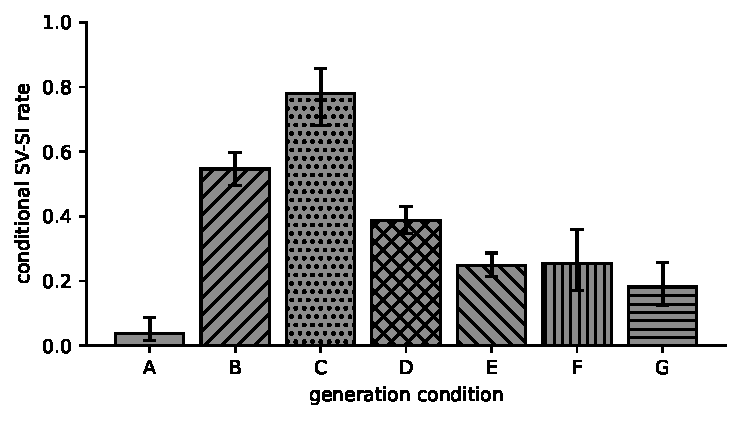
\includegraphics[width=\columnwidth]{../09_DIAGRAMS/rendered/fig_svsi_by_condition.pdf}
\caption{Conditional SV-SI rate by generation condition with Wilson 95\,\% intervals, over decided
structural passes (P5 excluded). C is the designed adversarial condition. A and G are the
\ifreviewed human-curated\else AI-drafted\fi{} reference conditions for legitimate input.}
\label{fig:by-condition}
\end{figure}}{}

\subsection{Violation types (RQ4)}
\ifjudgeweak Counts of judgement-rule violations depend on the judge and are exploratory.\fi{}
Judgement-rule violations outnumber objective ones (\R{viol.jud} against \R{viol.obj}, across all
conditions). The single most frequent violation is objective: a workshop must start in the future
(\R{rule.B-CO-2}). It is followed by a profile bio addressed to the assistant (\R{rule.B-PR-6}), a
ticket priority inconsistent with its text (\R{rule.B-TK-4}) and duration plausibility
(\R{rule.B-CO-3}). The ticket rule was judged without the text it depends on. On AI-facing fields,
\R{ai.llm.svsi} structurally valid LLM inputs violated a rule. Of those, \R{ai.llm.p5} came from the
injection family and \R{ai.llm.nonp5} from the other prompt families.

\subsection{Ground-truth agreement}
\ifhumanlabels On judgement rules, the judge agreed with the human annotator on \R{agree.judge}\,\% of
\R{n.judge} rule verdicts where both gave a verdict (Cohen's $\kappa=\R{kappa.judge}$); the annotator
was unsure on \R{unsure.judge}\,\% of judgement-rule verdicts. \ifjudgeweak Agreement is below the
pre-registered 0.4, so every judgement-rule result in this paper is exploratory.\else Agreement meets
the pre-registered 0.4 threshold.\fi{} The rule functions agreed with the annotator on
\R{agree.rules}\,\% of objective-rule verdicts ($\kappa=\R{kappa.rules}$), and the annotator's
repeated annotations agreed with each other on \R{agree.self}\,\% ($\kappa=\R{kappa.self}$). The
objective-rule results below are decided by those rule functions rather than by the judge, but that
single human check of them is itself weak, so they are better described as independent of the judge
than as externally validated.\else
Judge--human agreement is not reported, because the human annotation was not completed
(\texttt{TODO-HUMAN}); judgement-rule results therefore rest on the judge alone. Objective-rule
results, which cover every structurally valid input, do not.\fi

\subsection{Detection quality (RQ5)}
\IfFileExists{tables/tab_detection.tex}{\begin{table*}[t]
\caption{Detection quality of the candidate semantic validation layers on the shared stratified sample
of 579 decided inputs (236 SV-SI, 343 valid), leave-fields-out (5 folds). Recall, 95\% bootstrap
interval, FPR and precision are at the pre-registered operating point: the threshold is the smallest
score whose false-positive rate on valid training-fold inputs is at most 5\%, applied to held-out fields.
AUROC is threshold-free. The native column (exploratory, not pre-registered) applies each design's own
decision rule without tuning: for SLM and JUDGE, the model answered ``not appropriate''; for R, EMB and
HYB, score $\geq 0.5$. JUDGE returned no usable verdict for 25\% of inputs, counted as not flagged. R's zero FPR is partly by construction: its rule
functions also decide the ground truth for objective rules. JUDGE shares a model family with the
generator and is a reference point. Latency is the median decision time of the layer alone on the study CPU;
HYB's figure reuses embeddings already cached by EMB, so its uncached request-path cost is the one in Table~\ref{tab:e4}.}
\label{tab:detection}
\centering
\begin{tabular}{lrrrrrrr}
\toprule
Design & Recall (\%) & 95\% CI & FPR (\%) & Precision (\%) & AUROC & Native recall / FPR (\%) & Median (ms) \\
\midrule
HYB & 27.1 & [21.8, 32.7] & 5.8 & 76.2 & 0.60 & 24.2 / 2.3 & 0.01 \\
JUDGE & 23.7 & [19.0, 29.1] & 3.5 & 82.4 & 0.76 & 51.7 / 6.7 & 2706 \\
R & 22.5 & [17.2, 27.8] & 0.0 & 100.0 & 0.61 & 22.5 / 0.0 & 0.01 \\
EMB & 4.7 & [2.1, 7.6] & 5.8 & 35.5 & 0.45 & 1.7 / 2.3 & 31 \\
SLM & 1.3 & [0.0, 3.0] & 1.2 & 42.9 & 0.75 & 69.1 / 20.4 & 1075 \\
\bottomrule
\end{tabular}
\end{table*}
}{}

No design reached the target, so H5 is not supported (Table~\ref{tab:detection}).\ifjudgeweak{}
Detection is measured against the same labels, so the judgement-rule part of these results is
exploratory as well. The objective-rule part is not.\fi{} At the operating point fixed on the training
folds, the best non-judge design, HYB, detected \R{e3.HYB.recall}\,\% of SV-SI inputs (CI
\R{e3.HYB.ci}) at a held-out FPR of \R{e3.HYB.fpr}\,\%, which is above the 5\,\% it was tuned for. Most
of what it catches comes from R. HYB and R both caught \R{e3.HYB.robj}\,\% of the inputs that violate
only objective rules, and \R{e3.HYB.rjud}\,\% and \R{e3.R.rjud}\,\% of those that violate a judgement
rule. On all decided inputs the fast designs reach \R{e3.R.fullrecall}\,\% for R and
\R{e3.HYB.fullrecall}\,\% for HYB. EMB on its own was no better than chance (AUROC
\R{e3.EMB.auroc}).

The prompted designs rank inputs better, with AUROC \R{e3.SLM.auroc} for SLM and \R{e3.JUDGE.auroc} for
JUDGE against \R{e3.HYB.auroc} for HYB. Their scores take only a handful of values, so holding FPR to
5\,\% on the training fields forces the threshold to the top confidence level. There SLM detects
\R{e3.SLM.recall}\,\% and JUDGE \R{e3.JUDGE.recall}\,\%. Taking each model's own verdict without
tuning, which is exploratory, SLM detects \R{e3.SLM.nrecall}\,\% while flagging \R{e3.SLM.nfpr}\,\% of
valid inputs, and JUDGE detects \R{e3.JUDGE.nrecall}\,\% while flagging \R{e3.JUDGE.nfpr}\,\%. JUDGE
gave no usable verdict for \R{e3.JUDGE.noverdict}\,\% of inputs. These designs receive a rubric similar
to the ground-truth judge's, so their agreement with it partly measures agreement between two LLMs.
Thresholds did not transfer across fields, and the held-out FPR per fold reached
\R{e3.emb.foldfprmax}\,\% for the embedding-based designs. On benign-unusual inputs the FPR at the
operating point was \R{e3.HYB.fprG}\,\% for HYB, \R{e3.SLM.fprG}\,\% for SLM and \R{e3.JUDGE.fprG}\,\%
for JUDGE.

\subsection{Overhead (RQ6)}
\IfFileExists{tables/tab_e4.tex}{\begin{table}[t]
\caption{Request-path overhead of each configuration (production build, four-core CPU, no GPU). Each
value is the median over three 60\,s runs, given as the range across the three endpoints (profile,
review, course). Added latency is relative to structural-only validation on the same endpoint and
concurrency. H6 is evaluated on the added p97.5, the nearest tail percentile the load generator reports.
``Ok'' is the share of layer calls that returned a verdict rather than failing open. ``$>$60\,000'': the configuration saturated, completing no request within at least two of
the three runs. Per-endpoint values are in the repository.}
\label{tab:e4}
\centering
\footnotesize
\setlength{\tabcolsep}{2pt}
\begin{tabular}{lrrrrl}
\toprule
Config. & $\Delta$p50 (ms) & $\Delta$p97.5 (ms) & req/s & Ok (\%) & H6 \\
\midrule
\multicolumn{6}{l}{\emph{Concurrency 1}} \\
structural & 0 & 0 & 42.9--47.4 & -- &  \\
R & 0--2 & 0--1 & 41.9--46.0 & 100 & holds \\
EMB & 27--48 & 65--96 & 13.2--19.2 & 100 & fails \\
HYB & 26--45 & 65--82 & 13.6--19.2 & 100 &  \\
SLM & 527--534 & 655--761 & 1.7--1.8 & 100 &  \\
JUDGE & 1611--7704 & 7683--10824 & 0.1--0.5 & 100 & holds \\
\multicolumn{6}{l}{\emph{Concurrency 8}} \\
structural & 0 & 0 & 41.7--48.3 & -- &  \\
R & 2--6 & -136--14 & 43.9--47.6 & 100 & holds \\
EMB & 126--288 & 122--751 & 16.0--27.9 & 100 & fails \\
HYB & 103--270 & 131--396 & 17.7--29.0 & 100 &  \\
SLM & 4149--4210 & 6780--7180 & 1.7--1.7 & 100 &  \\
JUDGE & 14282--$>$60\,000 & 23474--$>$60\,000 & 0.0--0.4 & 100 & holds \\
\bottomrule
\end{tabular}
\end{table}
}{}

Each configuration ran against the production build with only its own model loaded. No request failed
and no layer call failed in any run (Table~\ref{tab:e4}). H6 is not supported, because its first part
fails. R added at most \R{e4.R.c1.maxadd}\,ms to p97.5 latency with one client and
\R{e4.R.c8.maxadd}\,ms with eight, which is within the 50\,ms bound. The negative differences at eight
clients reflect run-to-run variation. EMB added
\R{e4.EMB.c1.minadd}--\R{e4.EMB.c1.maxadd}\,ms with one client, above the bound, and
\R{e4.EMB.c8.minadd}--\R{e4.EMB.c8.maxadd}\,ms with eight, because every request embeds its text on the
same CPU. On the p95 bracket used as a sensitivity check, EMB fails on the review endpoint and is undetermined
on the other two. The second part of H6 holds. SLM added
\R{e4.SLM.c1.minp50add}--\R{e4.SLM.c1.maxp50add}\,ms at the median with one client and JUDGE added
\R{e4.JUDGE.c1.minp50add}--\R{e4.JUDGE.c1.maxp50add}\,ms. The model server answers one request at a
time, so requests queue under concurrency. With eight clients SLM added
\R{e4.SLM.c8.minp50add}--\R{e4.SLM.c8.maxp50add}\,ms at the median, and JUDGE completed no request
within the 60\,s window in all three runs on the course endpoint and in two of three on the review
endpoint. Throughput on the course endpoint fell from \R{e4.structural.c1.courses.rps} requests per
second with structural validation alone to \R{e4.SLM.c1.courses.rps} with SLM and
\R{e4.JUDGE.c1.courses.rps} with JUDGE. Set against detection quality (Fig.~\ref{fig:tradeoff}), only R
and HYB lie on the trade-off frontier. SLM, JUDGE and EMB each cost more and detect less than one of
them at the pre-registered operating point.

\IfFileExists{../09_DIAGRAMS/rendered/fig_tradeoff.pdf}{%
\begin{figure}[t]\centering
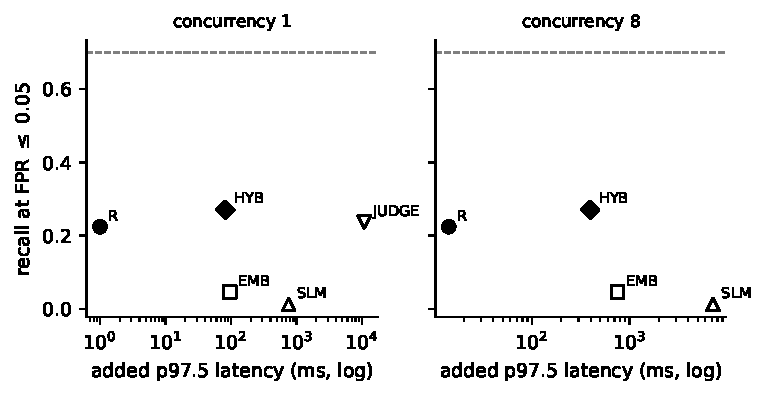
\includegraphics[width=\columnwidth]{../09_DIAGRAMS/rendered/fig_tradeoff.pdf}
\caption{Detection versus request-path cost for each semantic layer: recall at FPR $\leq$ 0.05 on
held-out fields (Table~\ref{tab:detection}) against the largest added p97.5 latency over the three
endpoints (Table~\ref{tab:e4}), per concurrency level. Filled markers lie on the trade-off frontier.
The dashed line is the pre-registered 70\,\% recall target. JUDGE at concurrency 8 saturated and is
drawn at its lower bound.}
\label{fig:tradeoff}
\end{figure}}{}

\section{Discussion}
\label{sec:discussion}

\ifjudgeweak Throughout this section, every statement that rests on judgement rules is exploratory,
because judge--human agreement fell below the pre-registered threshold. Statements about objective
rules do not depend on the judge.\fi

\textbf{RQ1: the gap is measurable, and its size depends on what is asked.} About a third of
structurally valid LLM inputs broke an unenforced rule. The figure is a fifth when the model was asked
only for legitimate values, and under a tenth on objective rules alone. This extends output-side
findings~\cite{li2026orderbench,singh2026sob,wrenn2026enterprise} to inputs that an application would
store. The magnitude is sensitive to prompt intent, to one date-dependent target, and to
\ifhumanlabels the judge, whose agreement with a human annotator was $\kappa=\R{kappa.judge}$\else an
unvalidated judge\fi. The claim that survives every check is that the gap is above the 5\,\% bound,
not any single figure.

\textbf{RQ2: where it occurs is uneven.} Category is moderately associated with the outcome, but
individual targets drive that association. One target with a clock-dependent rule accounts for over
half of the cross-field violations, and the structured category is a single target that the judge
scored without its context.

\textbf{RQ3: the gap is not specific to AI.} This is the central negative result. Random values that
satisfy the schema broke rules more often than model values, with or without field context, both pooled
and within target. The results point to the validation boundary rather than to the producer. A schema
admits many values the application should reject, and any producer that satisfies the schema without
knowing the rules will supply some of them. What distinguishes the model is that context helps. Giving
it the purpose and the rules cut the odds of a violation by \R{cmh.EvD.reduction}\,\% relative to the
schema alone. The random generator produces word sequences with no attempt at meaning, so it is a weak
producer, and the comparison bounds non-AI input rather than characterising it.

\textbf{RQ4: most violations are ordinary.} The single most frequent violation was of an objective rule
that the application could enforce directly, so enforcing objective rules would remove part of the gap.
Judgement-rule violations are still the majority. On AI-facing fields most LLM violations came from
ordinary prompts rather than from injection attempts, so the gap is mostly unenforced business logic
rather than attack.

\textbf{RQ5: no cheap layer closes it.} The fast designs that can be held to a low FPR, R and HYB, find
about a quarter of the violations at the operating point, and most of what they find are objective
violations that could simply be enforced. JUDGE at a similar FPR also finds about a quarter, split
evenly between objective and judgement rules. The prompted models discriminate better but produce
coarse, field-dependent scores. Used as they are, they catch more while rejecting between one valid
input in fifteen and one in five in this sample. Detecting judgement-rule violations remains the open
problem.

\textbf{RQ6: cost rises faster than detection.} On commodity CPU hardware only the rule layer is
effectively free, and it detects violations of rules the application could have enforced in the first
place. The embedding layer costs tens of milliseconds per request and detected almost nothing here. The
prompted models cost half a second to several seconds per request with one client, and a local model
server handles one request at a time, so they cannot keep up with eight. Their better ranking of inputs
does not survive the false-positive constraint. On this hardware the practical recommendation is to
enforce objective rules in code and to treat judgement rules as an open problem, rather than to add a
model to the request path.

\textbf{Alternative explanations.} The six explanations fixed in advance fare as follows. \emph{Weak
business rules rather than AI:} consistent with the data, because the gap appears for every producer
that does not know the rules. \emph{Random inputs produce the same effect:} consistent, and random
inputs exceed model inputs. \emph{Unusual human inputs behave the same:} \ifreviewed not resolved.
Human-curated unusual inputs did not differ detectably from context-aware model inputs
(\R{cmh.EvG.or}, \R{cmh.EvG.ci}), but the interval spans both directions and the contrast is
exploratory\else not tested, because the reference inputs are AI-drafted\fi. \emph{Confined to free
text:} not supported, because structured and cross-field targets also show high rates, although single
targets drive them. \emph{Prompt injection under another name:} not supported. Injection prompts are
excluded from all rates and account for \R{ai.llm.p5} of \R{ai.llm.svsi} LLM violations on AI-facing
fields. \emph{Too expensive to deploy:} supported for the model-based layers on CPU hardware, and not
supported for rules.

\section{Threats to Validity}
\label{sec:threats}

\textbf{Internal validity.} Labelling is the main threat. Judgement rules were decided by one 4B judge
\ifhumanlabels (agreement with a human annotator $\kappa=\R{kappa.judge}$ on \R{n.judge} shared
verdicts, below the pre-registered 0.4, so judgement-rule results are exploratory)\else without human
validation\fi, and seven of them were decided without the fields they depend on. Excluding those seven
lowers the LLM rate to \R{s.llm.nocontext}\,\% and lowers the random rate by more
(Table~\ref{tab:sensitivity}), which leaves the RQ3 direction intact. Agreement on semantic judgements
can be low even between humans~\cite{calo2026semanticgap}.\ifhumanlabels{} The disagreement here is not
one-sided noise. On the shared verdicts the judge called \R{fail.other.judge} violations against the
annotator's \R{fail.human.judge}, so the judge is the stricter rater and judgement-rule rates may be
too high. The judge also returned no usable verdict on \R{noverdict.judge} further rules that the
annotator decided, and the agreement statistic cannot use those. The annotator in turn disagreed with
the deterministic rule functions on objective rules ($\kappa=\R{kappa.rules}$, \R{agree.rules}\,\%
agreement, \R{fail.other.rules} rule-function violations against \R{fail.human.rules}), and those
functions decide such rules from the record and the clock. Part of the low agreement is therefore
annotation error, or the limited context the annotator was shown, rather than judge error alone. The
annotator was self-consistent on the repeated items ($\kappa=\R{kappa.self}$).\fi{} The judge sample
gives the conditions different target mixes, and target-weighted rates are close to the pooled ones.
Values generated in one call are correlated, so the intervals understate uncertainty. Time-relative
rules are evaluated against the clock at the moment the labels are merged, so a later re-run can change
labels near the boundary. The judge ran once, and its run-to-run stability on this CPU was not
measured.

\textbf{Defects found and corrected.} Six defects were found during execution, and each is recorded as
a deviation with the invalid data preserved. (i) The database was not reset between booking
measurements, so course capacity ran out. Bookings are now reset before each measurement and the
booking targets were re-measured. (ii) A resume routine retried failed generation calls, and the
retried records are excluded. (iii) Model outputs with other key names were silently replaced by form
defaults, and those records are excluded as generation failures. (iv) A first overhead run never
enabled the layer, and it is discarded. (v) The first detector analysis selected thresholds with a
quantile, which fails for coarse scores, and it was replaced before any detector result was reported.
(vi) The label merge never passed human verdicts to the ground-truth algorithm, and the label importer
dropped cells after an empty one. Both were found and fixed before the human annotation was collected,
and the annotation was imported with the corrected code. Defects (iii), (v) and (vi) were found by
independent review of the analysis and the code.

\textbf{External validity.} The study covers one application in one domain, built by the researcher,
with one enforcement profile, so the results may not transfer. Generation uses quantised open models of
1.7 to 8 billion parameters on CPU. Frontier models may behave differently, and the evidence that scale
does not predict semantic quality~\cite{singh2026sob,wrenn2026enterprise} cuts both ways. The prompts
never state the current date, which inflates date-rule violations for model inputs.

\textbf{Construct validity.} Semantic invalidity is defined by a frozen reference that another team
would write differently. The reference was frozen before any input existed, and violations are reported
per rule, so a reader can discount rules they disagree with.

\textbf{Conclusion validity.} Pooling three runs inflates the LLM sample, and per-run rates are
reported for that reason. The category mapping assigns dual-tagged fields to one category, which was
decided before the data existed but not logged at the time. The three contrasts H3a to H3c were the
only pre-declared ones, but they are computed on labels that include judgement rules,
so\ifjudgeweak{} they too are exploratory under the pre-registered agreement gate, and only results
decided by the rule functions alone remain confirmatory.\else{} they remain confirmatory while the
other contrasts are exploratory.\fi

\textbf{Who produced the human data.} \ifhumanlabels The reviewer and the annotator were the same
person, the author, who also built the subject application and wrote the rule reference. The annotation
is blind to the generation condition, because the interface never shows it, but it is not independent
of the study, and a single annotator cannot establish how far the disagreement with the judge
generalises. The review took \R{review.minutes} minutes for \R{e1.refdrafted} values, a median of
\R{review.median_s}\,s per value, and the annotation took \R{ann.minutes} minutes for \R{ann.items}
items, a median of \R{ann.median_s}\,s per item. Both are well below the effort budgeted for them,
which may itself contribute to the low agreement. The per-item answers and their timestamps are
released with the artefacts.\else The human tasks have not been carried out.\fi

\textbf{Provenance.} The reference conditions A and G were specified as human-written and were drafted
by an AI assistant. \ifreviewed A human reviewer then reviewed and curated them, so H3b compares model
input with human-curated input rather than with input a person wrote unaided. H3b remains exploratory
because it depends on judgement rules.\else Until the researcher's review is recorded, H3b is
exploratory and the alternative explanation that unusual human inputs behave similarly is not
tested.\fi

\section{Conclusion and Future Work}
\label{sec:conclusion}

Schema validation answers whether an input is well formed, not whether it belongs. At the input
boundary of one application with an explicit rule reference, about a third of structurally valid LLM
inputs broke an unenforced business rule. Random structurally valid inputs broke rules more often, and
telling the model the field's purpose and rules reduced violations. The gap is therefore a property of
what the application leaves unenforced and is not specific to AI-generated input. The single most
frequent violation was of an objective rule that a line of validation code could enforce. None of the
five candidate layers detected the pre-registered share of violations at a tolerable false-positive
rate.\ifjudgeweak{} A human annotation of \R{ann.items} inputs agreed with the judge only at
$\kappa=\R{kappa.judge}$, below the threshold fixed in advance, so every result that depends on
judgement rules is exploratory, and the ground truth for those rules is the weakest part of the
study.\fi{} On a four-core CPU, rules added at most \R{e4.R.c8.maxadd}\,ms at p97.5 and embeddings tens
of milliseconds. At the median a small language model added about half a second and an LLM judge
several seconds, and the judge saturated on two of three endpoints with eight concurrent clients.

Future work should \ifreviewed\else complete the review of the reference conditions, \fi
\ifhumanlabels\else validate the judge against human annotation, \fi strengthen the ground truth for
judgement rules with several annotators and more time per item, collect reference inputs written by
several people unaided, re-judge the context-dependent rules with the full record, state the current
date to the generators, and repeat the protocol on an existing open-source application.

\section*{Artifact Availability}

The testbed (tag \texttt{v1.0-frozen}), the harness, the prompts, the rule reference, every generated
input, measurement and label, and the scripts that produce every table, figure and number in this paper
are released with it (\texttt{TODO-HUMAN}: repository URL and licence).

\section*{Acknowledgment}

The literature search, verification, drafting, harness implementation and analysis scripting were
performed with the assistance of an AI system under the author's direction; the research claims and
the manuscript are the author's responsibility. A full disclosure of AI use and all artefacts are
released with the paper.

\bibliographystyle{IEEEtran}
\bibliography{references}

\end{document}
